
%% bare_jrnl_compsoc.tex
%% V1.4b
%% 2015/08/26
%% by Michael Shell
%% See:
%% http://www.michaelshell.org/
%% for current contact information.
%%
%% This is a skeleton file demonstrating the use of IEEEtran.cls
%% (requires IEEEtran.cls version 1.8b or later) with an IEEE
%% Computer Society journal paper.
%%
%% Support sites:
%% http://www.michaelshell.org/tex/ieeetran/
%% http://www.ctan.org/pkg/ieeetran
%% and
%% http://www.ieee.org/

%%*************************************************************************
%% Legal Notice:
%% This code is offered as-is without any warranty either expressed or
%% implied; without even the implied warranty of MERCHANTABILITY or
%% FITNESS FOR A PARTICULAR PURPOSE! 
%% User assumes all risk.
%% In no event shall the IEEE or any contributor to this code be liable for
%% any damages or losses, including, but not limited to, incidental,
%% consequential, or any other damages, resulting from the use or misuse
%% of any information contained here.
%%
%% All comments are the opinions of their respective authors and are not
%% necessarily endorsed by the IEEE.
%%
%% This work is distributed under the LaTeX Project Public License (LPPL)
%% ( http://www.latex-project.org/ ) version 1.3, and may be freely used,
%% distributed and modified. A copy of the LPPL, version 1.3, is included
%% in the base LaTeX documentation of all distributions of LaTeX released
%% 2003/12/01 or later.
%% Retain all contribution notices and credits.
%% ** Modified files should be clearly indicated as such, including  **
%% ** renaming them and changing author support contact information. **
%%*************************************************************************


% *** Authors should verify (and, if needed, correct) their LaTeX system  ***
% *** with the testflow diagnostic prior to trusting their LaTeX platform ***
% *** with production work. The IEEE's font choices and paper sizes can   ***
% *** trigger bugs that do not appear when using other class files.       ***                          ***
% The testflow support page is at:
% http://www.michaelshell.org/tex/testflow/


\documentclass[10pt,journal,compsoc]{IEEEtran}
%
% If IEEEtran.cls has not been installed into the LaTeX system files,
% manually specify the path to it like:
% \documentclass[10pt,journal,compsoc]{../sty/IEEEtran}





% Some very useful LaTeX packages include:
% (uncomment the ones you want to load)


% *** MISC UTILITY PACKAGES ***
%
%\usepackage{ifpdf}
% Heiko Oberdiek's ifpdf.sty is very useful if you need conditional
% compilation based on whether the output is pdf or dvi.
% usage:
% \ifpdf
%   % pdf code
% \else
%   % dvi code
% \fi
% The latest version of ifpdf.sty can be obtained from:
% http://www.ctan.org/pkg/ifpdf
% Also, note that IEEEtran.cls V1.7 and later provides a builtin
% \ifCLASSINFOpdf conditional that works the same way.
% When switching from latex to pdflatex and vice-versa, the compiler may
% have to be run twice to clear warning/error messages.






% *** CITATION PACKAGES ***
%
\ifCLASSOPTIONcompsoc
  % IEEE Computer Society needs nocompress option
  % requires cite.sty v4.0 or later (November 2003)
  \usepackage[nocompress]{cite}
\else
  % normal IEEE
  \usepackage{cite}
\fi
% cite.sty was written by Donald Arseneau
% V1.6 and later of IEEEtran pre-defines the format of the cite.sty package
% \cite{} output to follow that of the IEEE. Loading the cite package will
% result in citation numbers being automatically sorted and properly
% "compressed/ranged". e.g., [1], [9], [2], [7], [5], [6] without using
% cite.sty will become [1], [2], [5]--[7], [9] using cite.sty. cite.sty's
% \cite will automatically add leading space, if needed. Use cite.sty's
% noadjust option (cite.sty V3.8 and later) if you want to turn this off
% such as if a citation ever needs to be enclosed in parenthesis.
% cite.sty is already installed on most LaTeX systems. Be sure and use
% version 5.0 (2009-03-20) and later if using hyperref.sty.
% The latest version can be obtained at:
% http://www.ctan.org/pkg/cite
% The documentation is contained in the cite.sty file itself.
%
% Note that some packages require special options to format as the Computer
% Society requires. In particular, Computer Society  papers do not use
% compressed citation ranges as is done in typical IEEE papers
% (e.g., [1]-[4]). Instead, they list every citation separately in order
% (e.g., [1], [2], [3], [4]). To get the latter we need to load the cite
% package with the nocompress option which is supported by cite.sty v4.0
% and later. Note also the use of a CLASSOPTION conditional provided by
% IEEEtran.cls V1.7 and later.





% *** GRAPHICS RELATED PACKAGES ***
%
\ifCLASSINFOpdf
  % \usepackage[pdftex]{graphicx}
  % declare the path(s) where your graphic files are
  % \graphicspath{{../pdf/}{../jpeg/}}
  % and their extensions so you won't have to specify these with
  % every instance of \includegraphics
  % \DeclareGraphicsExtensions{.pdf,.jpeg,.png}
\else
  % or other class option (dvipsone, dvipdf, if not using dvips). graphicx
  % will default to the driver specified in the system graphics.cfg if no
  % driver is specified.
  % \usepackage[dvips]{graphicx}
  % declare the path(s) where your graphic files are
  % \graphicspath{{../eps/}}
  % and their extensions so you won't have to specify these with
  % every instance of \includegraphics
  % \DeclareGraphicsExtensions{.eps}
\fi
% graphicx was written by David Carlisle and Sebastian Rahtz. It is
% required if you want graphics, photos, etc. graphicx.sty is already
% installed on most LaTeX systems. The latest version and documentation
% can be obtained at: 
% http://www.ctan.org/pkg/graphicx
% Another good source of documentation is "Using Imported Graphics in
% LaTeX2e" by Keith Reckdahl which can be found at:
% http://www.ctan.org/pkg/epslatex
%
% latex, and pdflatex in dvi mode, support graphics in encapsulated
% postscript (.eps) format. pdflatex in pdf mode supports graphics
% in .pdf, .jpeg, .png and .mps (metapost) formats. Users should ensure
% that all non-photo figures use a vector format (.eps, .pdf, .mps) and
% not a bitmapped formats (.jpeg, .png). The IEEE frowns on bitmapped formats
% which can result in "jaggedy"/blurry rendering of lines and letters as
% well as large increases in file sizes.
%
% You can find documentation about the pdfTeX application at:
% http://www.tug.org/applications/pdftex






% *** MATH PACKAGES ***
%
%\usepackage{amsmath}
% A popular package from the American Mathematical Society that provides
% many useful and powerful commands for dealing with mathematics.
%
% Note that the amsmath package sets \interdisplaylinepenalty to 10000
% thus preventing page breaks from occurring within multiline equations. Use:
%\interdisplaylinepenalty=2500
% after loading amsmath to restore such page breaks as IEEEtran.cls normally
% does. amsmath.sty is already installed on most LaTeX systems. The latest
% version and documentation can be obtained at:
% http://www.ctan.org/pkg/amsmath





% *** SPECIALIZED LIST PACKAGES ***
%
%\usepackage{algorithmic}
% algorithmic.sty was written by Peter Williams and Rogerio Brito.
% This package provides an algorithmic environment fo describing algorithms.
% You can use the algorithmic environment in-text or within a figure
% environment to provide for a floating algorithm. Do NOT use the algorithm
% floating environment provided by algorithm.sty (by the same authors) or
% algorithm2e.sty (by Christophe Fiorio) as the IEEE does not use dedicated
% algorithm float types and packages that provide these will not provide
% correct IEEE style captions. The latest version and documentation of
% algorithmic.sty can be obtained at:
% http://www.ctan.org/pkg/algorithms
% Also of interest may be the (relatively newer and more customizable)
% algorithmicx.sty package by Szasz Janos:
% http://www.ctan.org/pkg/algorithmicx




% *** ALIGNMENT PACKAGES ***
%
%\usepackage{array}
% Frank Mittelbach's and David Carlisle's array.sty patches and improves
% the standard LaTeX2e array and tabular environments to provide better
% appearance and additional user controls. As the default LaTeX2e table
% generation code is lacking to the point of almost being broken with
% respect to the quality of the end results, all users are strongly
% advised to use an enhanced (at the very least that provided by array.sty)
% set of table tools. array.sty is already installed on most systems. The
% latest version and documentation can be obtained at:
% http://www.ctan.org/pkg/array


% IEEEtran contains the IEEEeqnarray family of commands that can be used to
% generate multiline equations as well as matrices, tables, etc., of high
% quality.




% *** SUBFIGURE PACKAGES ***
%\ifCLASSOPTIONcompsoc
%  \usepackage[caption=false,font=footnotesize,labelfont=sf,textfont=sf]{subfig}
%\else
%  \usepackage[caption=false,font=footnotesize]{subfig}
%\fi
% subfig.sty, written by Steven Douglas Cochran, is the modern replacement
% for subfigure.sty, the latter of which is no longer maintained and is
% incompatible with some LaTeX packages including fixltx2e. However,
% subfig.sty requires and automatically loads Axel Sommerfeldt's caption.sty
% which will override IEEEtran.cls' handling of captions and this will result
% in non-IEEE style figure/table captions. To prevent this problem, be sure
% and invoke subfig.sty's "caption=false" package option (available since
% subfig.sty version 1.3, 2005/06/28) as this is will preserve IEEEtran.cls
% handling of captions.
% Note that the Computer Society format requires a sans serif font rather
% than the serif font used in traditional IEEE formatting and thus the need
% to invoke different subfig.sty package options depending on whether
% compsoc mode has been enabled.
%
% The latest version and documentation of subfig.sty can be obtained at:
% http://www.ctan.org/pkg/subfig




% *** FLOAT PACKAGES ***
%
%\usepackage{fixltx2e}
% fixltx2e, the successor to the earlier fix2col.sty, was written by
% Frank Mittelbach and David Carlisle. This package corrects a few problems
% in the LaTeX2e kernel, the most notable of which is that in current
% LaTeX2e releases, the ordering of single and double column floats is not
% guaranteed to be preserved. Thus, an unpatched LaTeX2e can allow a
% single column figure to be placed prior to an earlier double column
% figure.
% Be aware that LaTeX2e kernels dated 2015 and later have fixltx2e.sty's
% corrections already built into the system in which case a warning will
% be issued if an attempt is made to load fixltx2e.sty as it is no longer
% needed.
% The latest version and documentation can be found at:
% http://www.ctan.org/pkg/fixltx2e


%\usepackage{stfloats}
% stfloats.sty was written by Sigitas Tolusis. This package gives LaTeX2e
% the ability to do double column floats at the bottom of the page as well
% as the top. (e.g., "\begin{figure*}[!b]" is not normally possible in
% LaTeX2e). It also provides a command:
%\fnbelowfloat
% to enable the placement of footnotes below bottom floats (the standard
% LaTeX2e kernel puts them above bottom floats). This is an invasive package
% which rewrites many portions of the LaTeX2e float routines. It may not work
% with other packages that modify the LaTeX2e float routines. The latest
% version and documentation can be obtained at:
% http://www.ctan.org/pkg/stfloats
% Do not use the stfloats baselinefloat ability as the IEEE does not allow
% \baselineskip to stretch. Authors submitting work to the IEEE should note
% that the IEEE rarely uses double column equations and that authors should try
% to avoid such use. Do not be tempted to use the cuted.sty or midfloat.sty
% packages (also by Sigitas Tolusis) as the IEEE does not format its papers in
% such ways.
% Do not attempt to use stfloats with fixltx2e as they are incompatible.
% Instead, use Morten Hogholm'a dblfloatfix which combines the features
% of both fixltx2e and stfloats:
%
% \usepackage{dblfloatfix}
% The latest version can be found at:
% http://www.ctan.org/pkg/dblfloatfix




%\ifCLASSOPTIONcaptionsoff
%  \usepackage[nomarkers]{endfloat}
% \let\MYoriglatexcaption\caption
% \renewcommand{\caption}[2][\relax]{\MYoriglatexcaption[#2]{#2}}
%\fi
% endfloat.sty was written by James Darrell McCauley, Jeff Goldberg and 
% Axel Sommerfeldt. This package may be useful when used in conjunction with 
% IEEEtran.cls'  captionsoff option. Some IEEE journals/societies require that
% submissions have lists of figures/tables at the end of the paper and that
% figures/tables without any captions are placed on a page by themselves at
% the end of the document. If needed, the draftcls IEEEtran class option or
% \CLASSINPUTbaselinestretch interface can be used to increase the line
% spacing as well. Be sure and use the nomarkers option of endfloat to
% prevent endfloat from "marking" where the figures would have been placed
% in the text. The two hack lines of code above are a slight modification of
% that suggested by in the endfloat docs (section 8.4.1) to ensure that
% the full captions always appear in the list of figures/tables - even if
% the user used the short optional argument of \caption[]{}.
% IEEE papers do not typically make use of \caption[]'s optional argument,
% so this should not be an issue. A similar trick can be used to disable
% captions of packages such as subfig.sty that lack options to turn off
% the subcaptions:
% For subfig.sty:
% \let\MYorigsubfloat\subfloat
% \renewcommand{\subfloat}[2][\relax]{\MYorigsubfloat[]{#2}}
% However, the above trick will not work if both optional arguments of
% the \subfloat command are used. Furthermore, there needs to be a
% description of each subfigure *somewhere* and endfloat does not add
% subfigure captions to its list of figures. Thus, the best approach is to
% avoid the use of subfigure captions (many IEEE journals avoid them anyway)
% and instead reference/explain all the subfigures within the main caption.
% The latest version of endfloat.sty and its documentation can obtained at:
% http://www.ctan.org/pkg/endfloat
%
% The IEEEtran \ifCLASSOPTIONcaptionsoff conditional can also be used
% later in the document, say, to conditionally put the References on a 
% page by themselves.




% *** PDF, URL AND HYPERLINK PACKAGES ***
%
%\usepackage{url}
% url.sty was written by Donald Arseneau. It provides better support for
% handling and breaking URLs. url.sty is already installed on most LaTeX
% systems. The latest version and documentation can be obtained at:
% http://www.ctan.org/pkg/url
% Basically, \url{my_url_here}.


% *** Additional packages ***
\usepackage{makeidx}  % allows for indexgeneration
\makeindex
%
%
\usepackage[utf8]{inputenc}
\usepackage[english]{babel}      % chnage the used langauge here!!!
\usepackage[T1]{fontenc}
\usepackage{url}
%
% T1 fonts will be used to generate the final print and online PDFs,
% so please use T1 fonts in your manuscript whenever possible.
% Other font encondings may result in incorrect characters.
%
\usepackage{graphicx}
% correct colors for the hyperrefs
\usepackage[plainpages=false,hypertexnames=true,pdfnewwindow=true,backref=page,colorlinks=true,citecolor=blue,linkcolor=black,urlcolor=blue,filecolor=blue]{hyperref}
%
% additional (maybe useful) packages
\usepackage{amssymb}                % more math symbols
\usepackage{amsmath}                % better equations
\usepackage{booktabs}               % better tables
\usepackage[dvipsnames]{xcolor}     % more colors
\usepackage{spverbatim}             % verbatim with automatic line breaks
\usepackage{dsfont}                 % math fonts
\usepackage{csquotes}               % correct "" based on the used language
\usepackage{listings}               % source code
\usepackage{tikz}                   % custom (vector) graphics
\usetikzlibrary{shapes, arrows.meta, positioning, decorations.pathreplacing, trees, patterns, calligraphy}
\usepackage{mathtools}
\DeclarePairedDelimiter\ceil{\lceil}{\rceil}
\DeclarePairedDelimiter\floor{\lfloor}{\rfloor}
%
% pseudo-code
\usepackage{algorithm} 
\usepackage{algpseudocode} 
\newcommand{\algorithmautorefname}{Algorithmus}

% LstListing-Format ==========================================================
\lstdefinestyle{cpp}{
  language=C++,
  basicstyle=\small\ttfamily,
  frame=tb,
  xleftmargin=\parindent,
  keywordstyle=\color{blue},
  stringstyle=\color{red},
  commentstyle=\color{ForestGreen},
  framexleftmargin=5pt,
  framexrightmargin=5pt,
  framextopmargin=5pt,
  framexbottommargin=5pt,
  literate={~}{$\sim$}1
}

% macro definitions ==========================================================
% numbers -------------------------------------------------------------
\newcommand{\N}{{\mathbb{N}}}
\newcommand{\R}{{\mathbb{R}}}
\newcommand{\C}{{\mathbb{C}}}
\newcommand{\Z}{{\mathbb{Z}}}
\newcommand{\Q}{{\mathbb{Q}}}
\newcommand{\todo}[1]{\textcolor{red}{\textbf{//TODO: } #1}}
\newcommand{\code}[1]{\texttt{#1}}
\renewcommand{\O}{{\mathcal{O}}}
\newcommand\norm[1]{\lVert#1\rVert}
\newcommand\scprod[2]{\langle #1 , #2 \rangle}
\usepackage{wrapfig}
\usepackage{url}
\usepackage{xurl}
%
%
\def\myverzeichnis{.}
%
\numberwithin{equation}{section}
%
%

\usepackage{amsthm}

\usepackage{caption}
\usepackage{subcaption}

\theoremstyle{definition}
\newtheorem{definition}{Definition}

\theoremstyle{plain}
\newtheorem{corollary}{Corollary}

% images -----------------------------------------------------------------------
% #1 filename;  #2 Label;  #3 caption;  #4 short-caption
\newcommand{\image}[4]{%
  \begin{figure}[htbp]%
    \begin{center}%
      \includegraphics{#1}%
      \caption[#4]{#3}%
      \label{#2}%
    \end{center}%
  \end{figure}%
}

% image with a specific width -----------------------------------------------------------------
% #1 filename;  #2 width;  #3 Label;  #4 caption;  #5 short-caption
\newcommand{\imagewithwidth}[5]{
  \begin{figure}[htbp]%
    \begin{center}%
      \includegraphics[width=#2]{#1}%
      \caption[#5]{#4}%
      \label{#3}%
    \end{center}%
  \end{figure}
}

\renewcommand\IEEEkeywordsname{Keywords}

% *** Do not adjust lengths that control margins, column widths, etc. ***
% *** Do not use packages that alter fonts (such as pslatex).         ***
% There should be no need to do such things with IEEEtran.cls V1.6 and later.
% (Unless specifically asked to do so by the journal or conference you plan
% to submit to, of course. )


% correct bad hyphenation here
\hyphenation{optical networks semi-conductor}

\begin{document}
%
% paper title
% Titles are generally capitalized except for words such as a, an, and, as,
% at, but, by, for, in, nor, of, on, or, the, to and up, which are usually
% not capitalized unless they are the first or last word of the title.
% Linebreaks \\ can be used within to get better formatting as desired.
% Do not put math or special symbols in the title.
\title{Towards Real-Time Physics in a 2D Survival-Based Game}
%
%
% author names and IEEE memberships
% note positions of commas and nonbreaking spaces ( ~ ) LaTeX will not break
% a structure at a ~ so this keeps an author's name from being broken across
% two lines.
% use \thanks{} to gain access to the first footnote area
% a separate \thanks must be used for each paragraph as LaTeX2e's \thanks
% was not built to handle multiple paragraphs
%
%
%\IEEEcompsocitemizethanks is a special \thanks that produces the bulleted
% lists the Computer Society journals use for "first footnote" author
% affiliations. Use \IEEEcompsocthanksitem which works much like \item
% for each affiliation group. When not in compsoc mode,
% \IEEEcompsocitemizethanks becomes like \thanks and
% \IEEEcompsocthanksitem becomes a line break with idention. This
% facilitates dual compilation, although admittedly the differences in the
% desired content of \author between the different types of papers makes a
% one-size-fits-all approach a daunting prospect. For instance, compsoc 
% journal papers have the author affiliations above the "Manuscript
% received ..."  text while in non-compsoc journals this is reversed. Sigh.

\author{Bj\"orn Aheimer, Felix R\"ohr, Daniel Six, Aleksis Vezenkov, Anietta Weckauff% <-this % stops a space
\IEEEcompsocitemizethanks{\IEEEcompsocthanksitem The authors are in the B.Sc.~Informatik at the University of Stuttgart\protect\\
Examiner: Prof. Dr. Miriam Schulte, Univ. of Stgt., IPVS/SGS\protect\\
Supervisor: Carme Homs-Pons, M.Sc., Univ. of Stgt., IPVS/SGS
% note need leading \protect in front of \\ to get a newline within \thanks as
% \\ is fragile and will error, could use \hfil\break instead.
}}

% note the % following the last \IEEEmembership and also \thanks - 
% these prevent an unwanted space from occurring between the last author name
% and the end of the author line. i.e., if you had this:
% 
% \author{....lastname \thanks{...} \thanks{...} }
%                     ^------------^------------^----Do not want these spaces!
%
% a space would be appended to the last name and could cause every name on that
% line to be shifted left slightly. This is one of those "LaTeX things". For
% instance, "\textbf{A} \textbf{B}" will typeset as "A B" not "AB". To get
% "AB" then you have to do: "\textbf{A}\textbf{B}"
% \thanks is no different in this regard, so shield the last } of each \thanks
% that ends a line with a % and do not let a space in before the next \thanks.
% Spaces after \IEEEmembership other than the last one are OK (and needed) as
% you are supposed to have spaces between the names. For what it is worth,
% this is a minor point as most people would not even notice if the said evil
% space somehow managed to creep in.



% The paper headers
\markboth{Bachelor Research Project Computer Science 2024}%
{Submission}
% The only time the second header will appear is for the odd numbered pages
% after the title page when using the twoside option.
% 
% *** Note that you probably will NOT want to include the author's ***
% *** name in the headers of peer review papers.                   ***
% You can use \ifCLASSOPTIONpeerreview for conditional compilation here if
% you desire.



% The publisher's ID mark at the bottom of the page is less important with
% Computer Society journal papers as those publications place the marks
% outside of the main text columns and, therefore, unlike regular IEEE
% journals, the available text space is not reduced by their presence.
% If you want to put a publisher's ID mark on the page you can do it like
% this:
%\IEEEpubid{0000--0000/00\$00.00~\copyright~2015 IEEE}
% or like this to get the Computer Society new two part style.
%\IEEEpubid{\makebox[\columnwidth]{\hfill 0000--0000/00/\$00.00~\copyright~2015 IEEE}%
%\hspace{\columnsep}\makebox[\columnwidth]{Published by the IEEE Computer Society\hfill}}
% Remember, if you use this you must call \IEEEpubidadjcol in the second
% column for its text to clear the IEEEpubid mark (Computer Society jorunal
% papers don't need this extra clearance.)



% use for special paper notices
%\IEEEspecialpapernotice{(Invited Paper)}



% for Computer Society papers, we must declare the abstract and index terms
% PRIOR to the title within the \IEEEtitleabstractindextext IEEEtran
% command as these need to go into the title area created by \maketitle.
% As a general rule, do not put math, special symbols or citations
% in the abstract or keywords.
\IEEEtitleabstractindextext{%
\begin{abstract}
  Surviving Sarntal is an action-packed arcade endless runner.
  The player has to navigate a hiker through demanding terrain while dodging dangerous rockfall.
  The game is implemented in C++ using only a small number of libraries.
  Goal of the project is the design of a finished game following good software engineering practice with particular focus on creating a performant physics engine for rigid body simulation.
  This report explains our development approach, the game logic, and it discusses our findings in all stages from research, development to deployment.
\end{abstract}

% Note that keywords are not normally used for peerreview papers.
\begin{IEEEkeywords}
Game Development,
Hermite Splines, 
Rigid Body Simulation,
Physics Engine,
SAT,
Collision Handling, 
C++
\end{IEEEkeywords}}


% make the title area
\maketitle


% To allow for easy dual compilation without having to reenter the
% abstract/keywords data, the \IEEEtitleabstractindextext text will
% not be used in maketitle, but will appear (i.e., to be "transported")
% here as \IEEEdisplaynontitleabstractindextext when the compsoc 
% or transmag modes are not selected <OR> if conference mode is selected 
% - because all conference papers position the abstract like regular
% papers do.
\IEEEdisplaynontitleabstractindextext
% \IEEEdisplaynontitleabstractindextext has no effect when using
% compsoc or transmag under a non-conference mode.



% For peer review papers, you can put extra information on the cover
% page as needed:
% \ifCLASSOPTIONpeerreview
% \begin{center} \bfseries EDICS Category: 3-BBND \end{center}
% \fi
%
% For peerreview papers, this IEEEtran command inserts a page break and
% creates the second title. It will be ignored for other modes.
\IEEEpeerreviewmaketitle



%\IEEEraisesectionheading{\section{Introduction}\label{sec:introduction}}
% Computer Society journal (but not conference!) papers do something unusual
% with the very first section heading (almost always called "Introduction").
% They place it ABOVE the main text! IEEEtran.cls does not automatically do
% this for you, but you can achieve this effect with the provided
% \IEEEraisesectionheading{} command. Note the need to keep any \label that
% is to refer to the section immediately after \section in the above as
% \IEEEraisesectionheading puts \section within a raised box.




% The very first letter is a 2 line initial drop letter followed
% by the rest of the first word in caps (small caps for compsoc).
% 
% form to use if the first word consists of a single letter:
% \IEEEPARstart{A}{demo} file is ....
% 
% form to use if you need the single drop letter followed by
% normal text (unknown if ever used by the IEEE):
% \IEEEPARstart{A}{}demo file is ....
% 
% Some journals put the first two words in caps:
% \IEEEPARstart{T}{his demo} file is ....
% 
% Here we have the typical use of a "T" for an initial drop letter
% and "HIS" in caps to complete the first word.
% \IEEEPARstart{T}{his}

% You must have at least 2 lines in the paragraph with the drop letter
% (should never be an issue)







% needed in second column of first page if using \IEEEpubid
%\IEEEpubidadjcol



% An example of a floating figure using the graphicx package.
% Note that \label must occur AFTER (or within) \caption.
% For figures, \caption should occur after the \includegraphics.
% Note that IEEEtran v1.7 and later has special internal code that
% is designed to preserve the operation of \label within \caption
% even when the captionsoff option is in effect. However, because
% of issues like this, it may be the safest practice to put all your
% \label just after \caption rather than within \caption{}.
%
% Reminder: the "draftcls" or "draftclsnofoot", not "draft", class
% option should be used if it is desired that the figures are to be
% displayed while in draft mode.
%
%\begin{figure}[!t]
%\centering
%\includegraphics[width=2.5in]{myfigure}
% where an .eps filename suffix will be assumed under latex, 
% and a .pdf suffix will be assumed for pdflatex; or what has been declared
% via \DeclareGraphicsExtensions.
%\caption{Simulation results for the network.}
%\label{fig_sim}
%\end{figure}

% Note that the IEEE typically puts floats only at the top, even when this
% results in a large percentage of a column being occupied by floats.
% However, the Computer Society has been known to put floats at the bottom.


% An example of a double column floating figure using two subfigures.
% (The subfig.sty package must be loaded for this to work.)
% The subfigure \label commands are set within each subfloat command,
% and the \label for the overall figure must come after \caption.
% \hfil is used as a separator to get equal spacing.
% Watch out that the combined width of all the subfigures on a 
% line do not exceed the text width or a line break will occur.
%
%\begin{figure*}[!t]
%\centering
%\subfloat[Case I]{\includegraphics[width=2.5in]{box}%
%\label{fig_first_case}}
%\hfil
%\subfloat[Case II]{\includegraphics[width=2.5in]{box}%
%\label{fig_second_case}}
%\caption{Simulation results for the network.}
%\label{fig_sim}
%\end{figure*}
%
% Note that often IEEE papers with subfigures do not employ subfigure
% captions (using the optional argument to \subfloat[]), but instead will
% reference/describe all of them (a), (b), etc., within the main caption.
% Be aware that for subfig.sty to generate the (a), (b), etc., subfigure
% labels, the optional argument to \subfloat must be present. If a
% subcaption is not desired, just leave its contents blank,
% e.g., \subfloat[].


% An example of a floating table. Note that, for IEEE style tables, the
% \caption command should come BEFORE the table and, given that table
% captions serve much like titles, are usually capitalized except for words
% such as a, an, and, as, at, but, by, for, in, nor, of, on, or, the, to
% and up, which are usually not capitalized unless they are the first or
% last word of the caption. Table text will default to \footnotesize as
% the IEEE normally uses this smaller font for tables.
% The \label must come after \caption as always.
%
%\begin{table}[!t]
%% increase table row spacing, adjust to taste
%\renewcommand{\arraystretch}{1.3}
% if using array.sty, it might be a good idea to tweak the value of
% \extrarowheight as needed to properly center the text within the cells
%\caption{An Example of a Table}
%\label{table_example}
%\centering
%% Some packages, such as MDW tools, offer better commands for making tables
%% than the plain LaTeX2e tabular which is used here.
%\begin{tabular}{|c||c|}
%\hline
%One & Two\\
%\hline
%Three & Four\\
%\hline
%\end{tabular}
%\end{table}


% Note that the IEEE does not put floats in the very first column
% - or typically anywhere on the first page for that matter. Also,
% in-text middle ("here") positioning is typically not used, but it
% is allowed and encouraged for Computer Society conferences (but
% not Computer Society journals). Most IEEE journals/conferences use
% top floats exclusively. 
% Note that, LaTeX2e, unlike IEEE journals/conferences, places
% footnotes above bottom floats. This can be corrected via the
% \fnbelowfloat command of the stfloats package.


\begin{frame}{A New Game with an Old Soul}
    \begin{minipage}{\textwidth}
        \centering
        \begin{minipage}{.495\textwidth}
            \onslide<1-2>{
                \begin{figure}
                    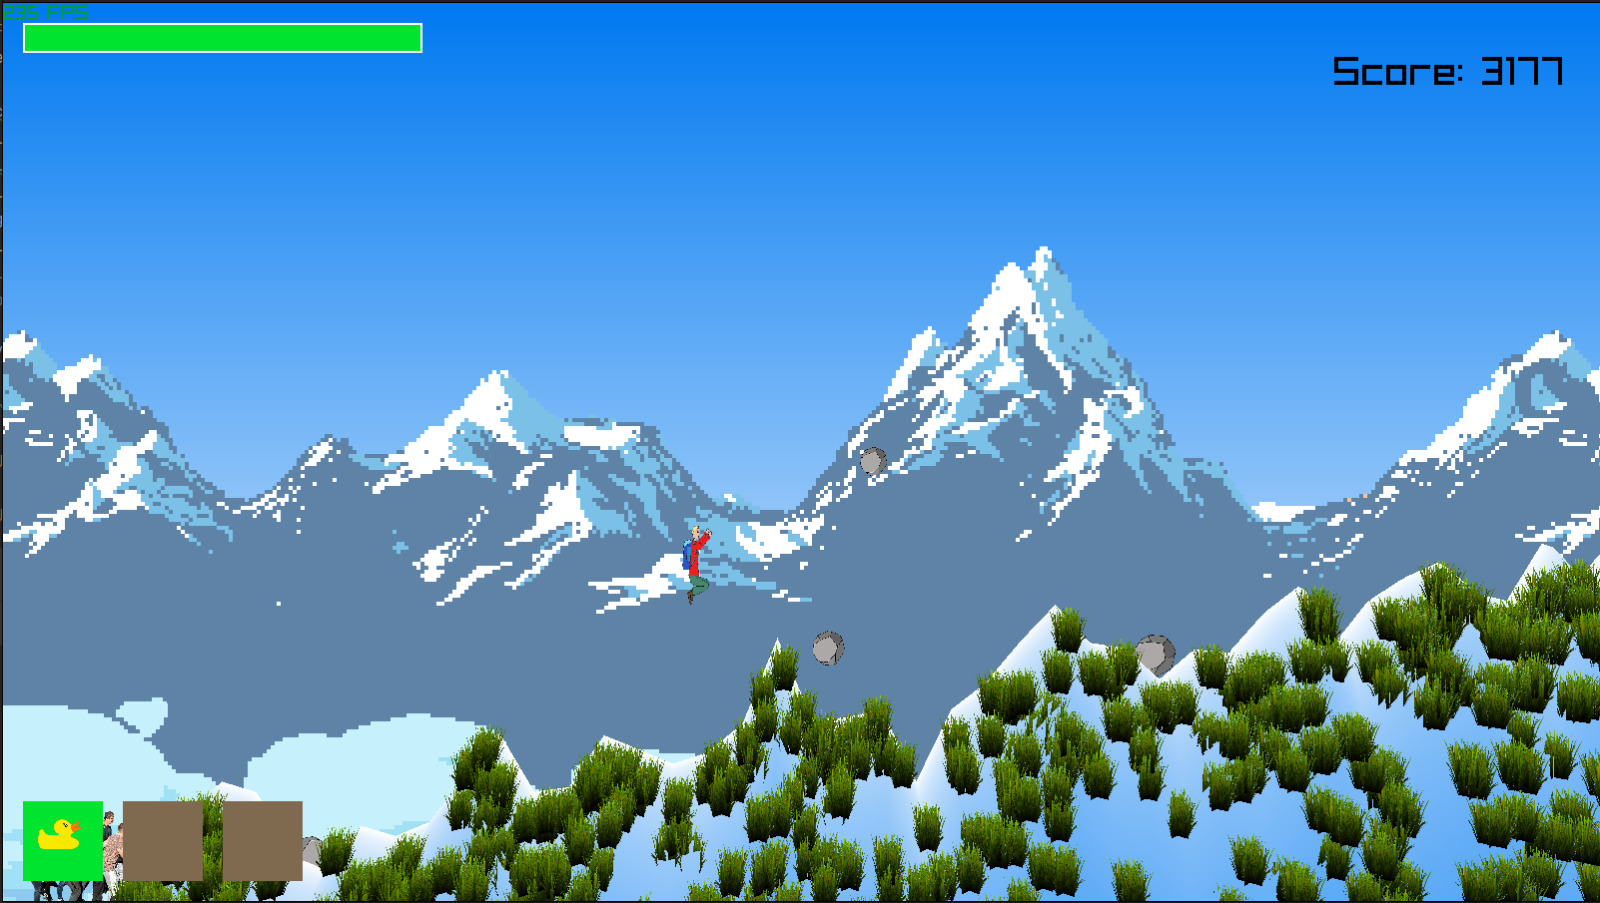
\includegraphics[width=\textwidth]{../figures/old_game.jpeg}
                    \caption{Ferienakademie 2023\phantom{y}}
                \end{figure}
            }
        \end{minipage}
        \begin{minipage}{.495\textwidth}
            \onslide<2>{
                \begin{figure}
                    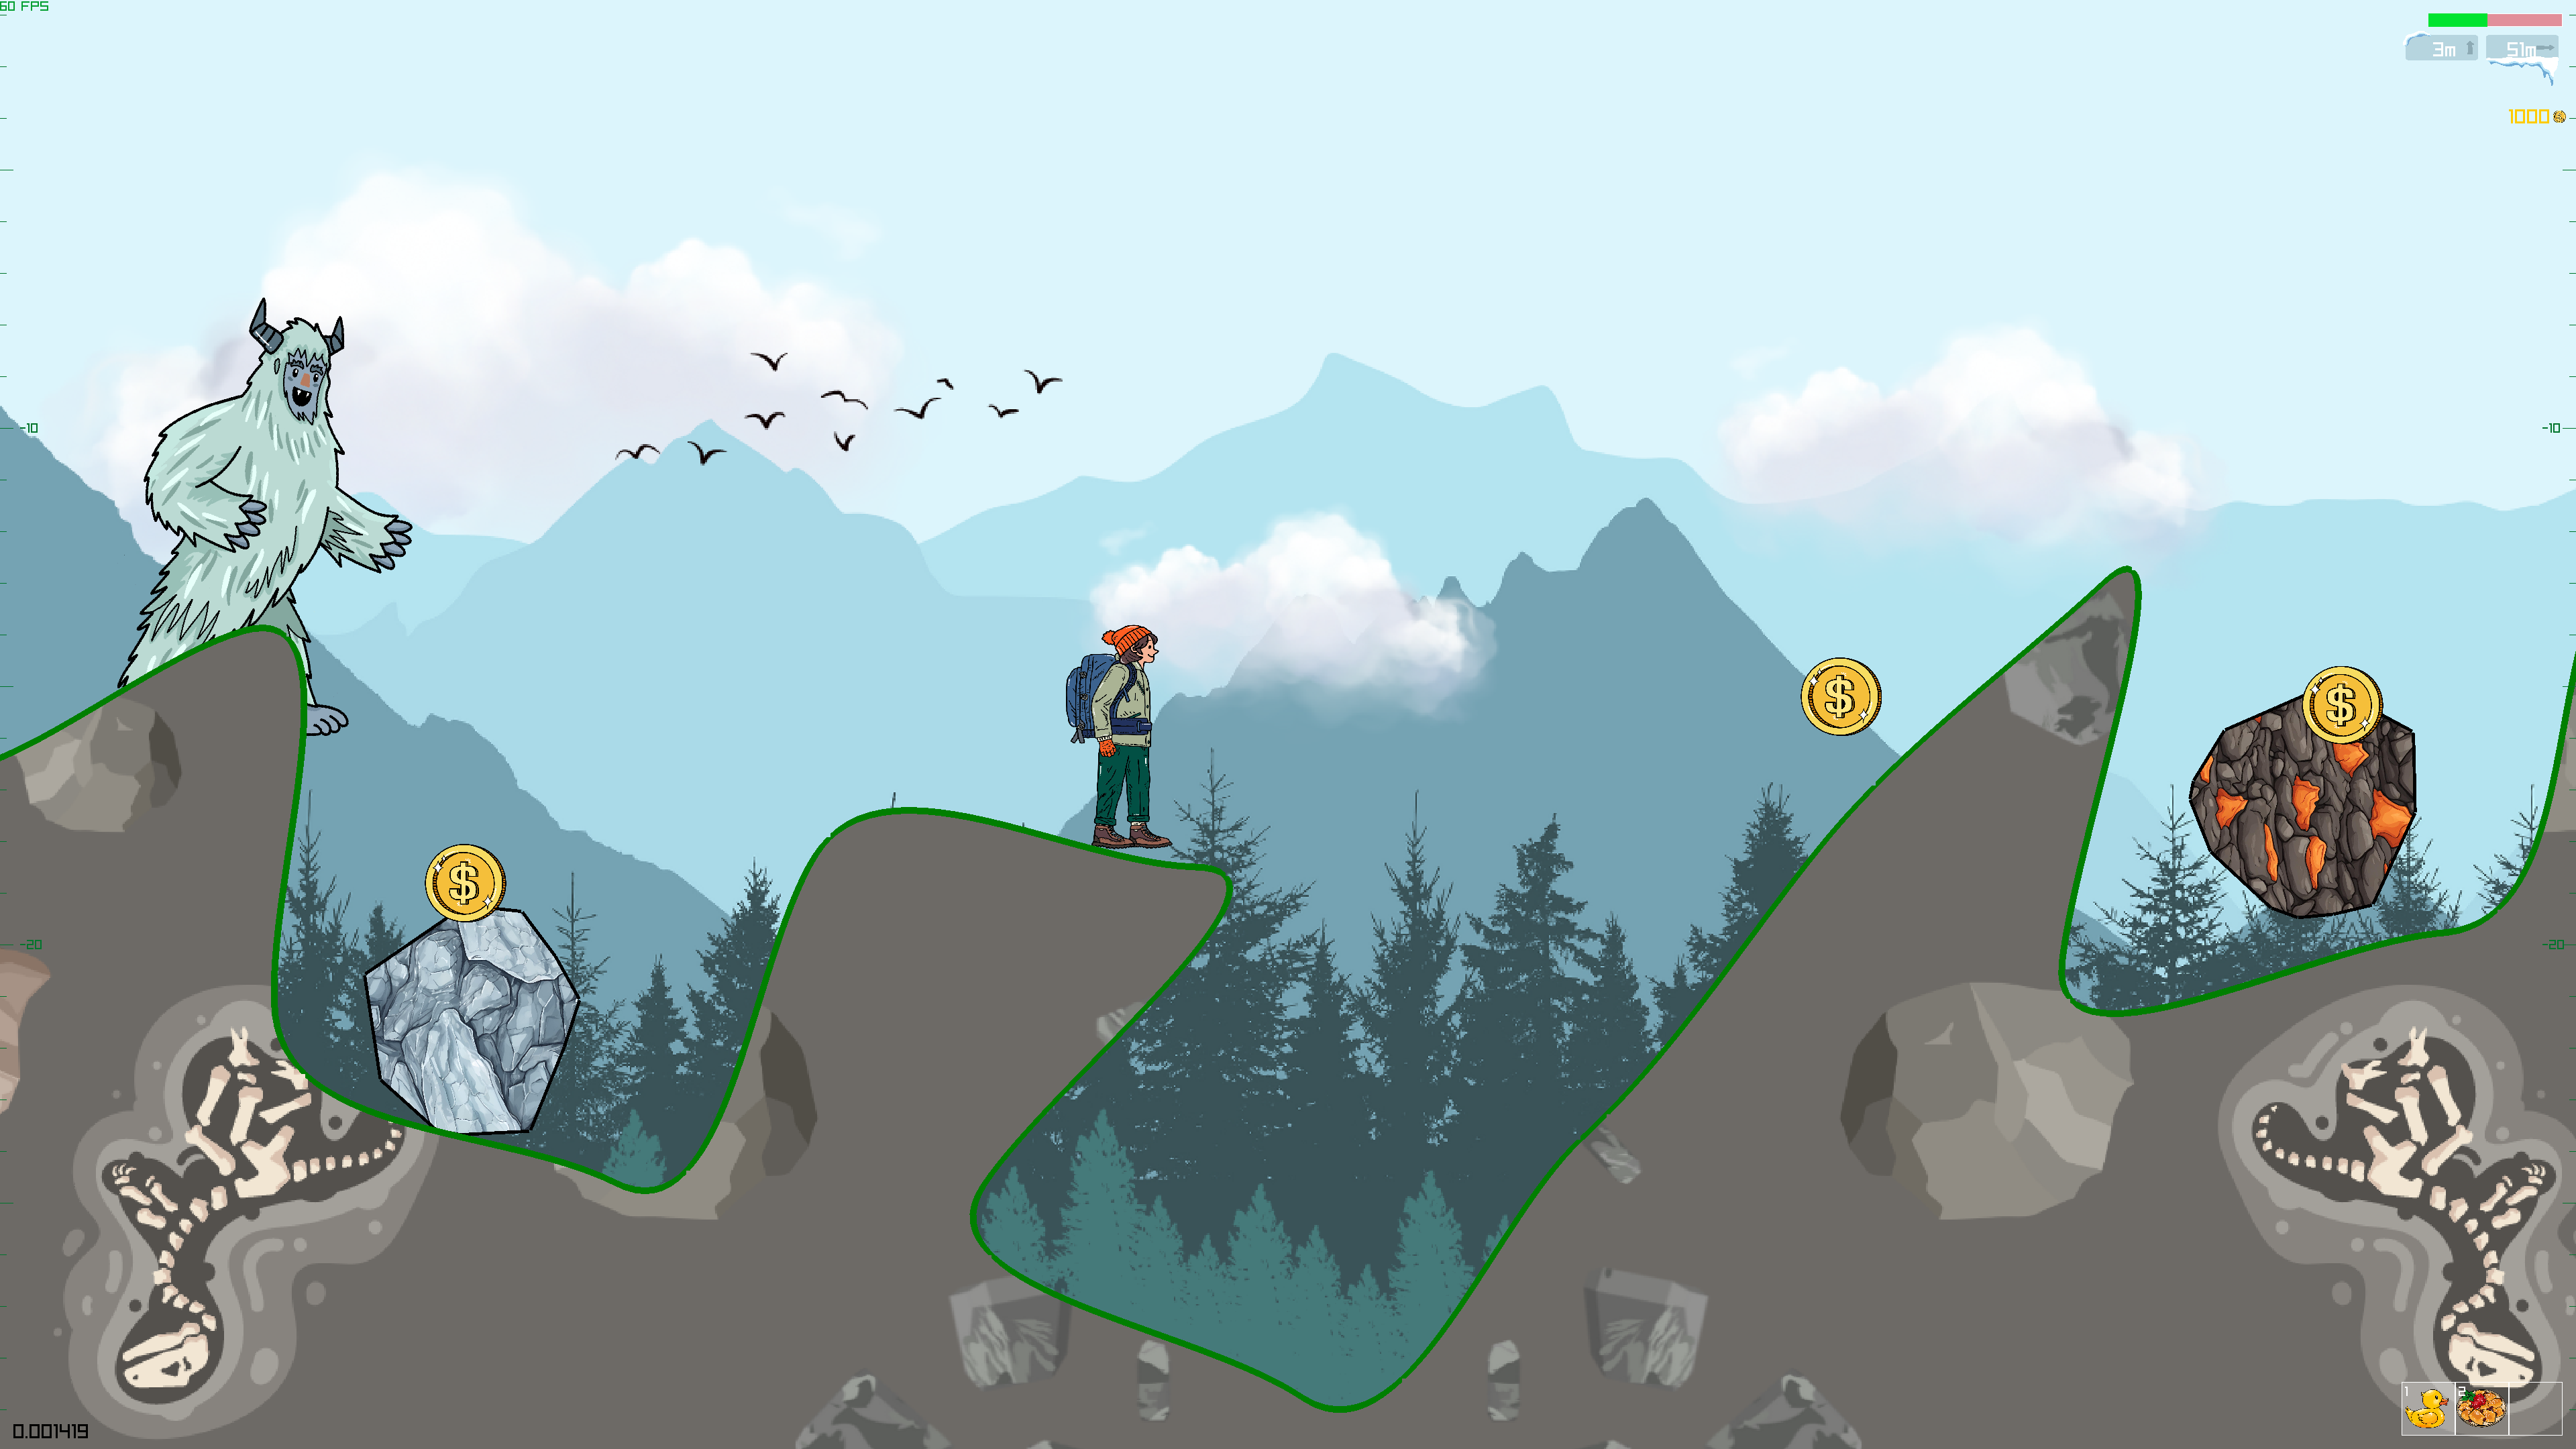
\includegraphics[width=\textwidth]{../figures/new_game.png}
                    \caption{Today}
                \end{figure}
            }
        \end{minipage}
    \end{minipage}
    %\vspace{-.45cm}
\end{frame}


\begin{frame}{Outline}
    \tableofcontents
\end{frame}


\begin{frame}{Introduction}
    \begin{itemize}
        \item Project objective: Enhance "Surviving Sarntal" with modular code, real-time physics, and improved user experience.
    \end{itemize}
    \centering
    \begin{figure}
        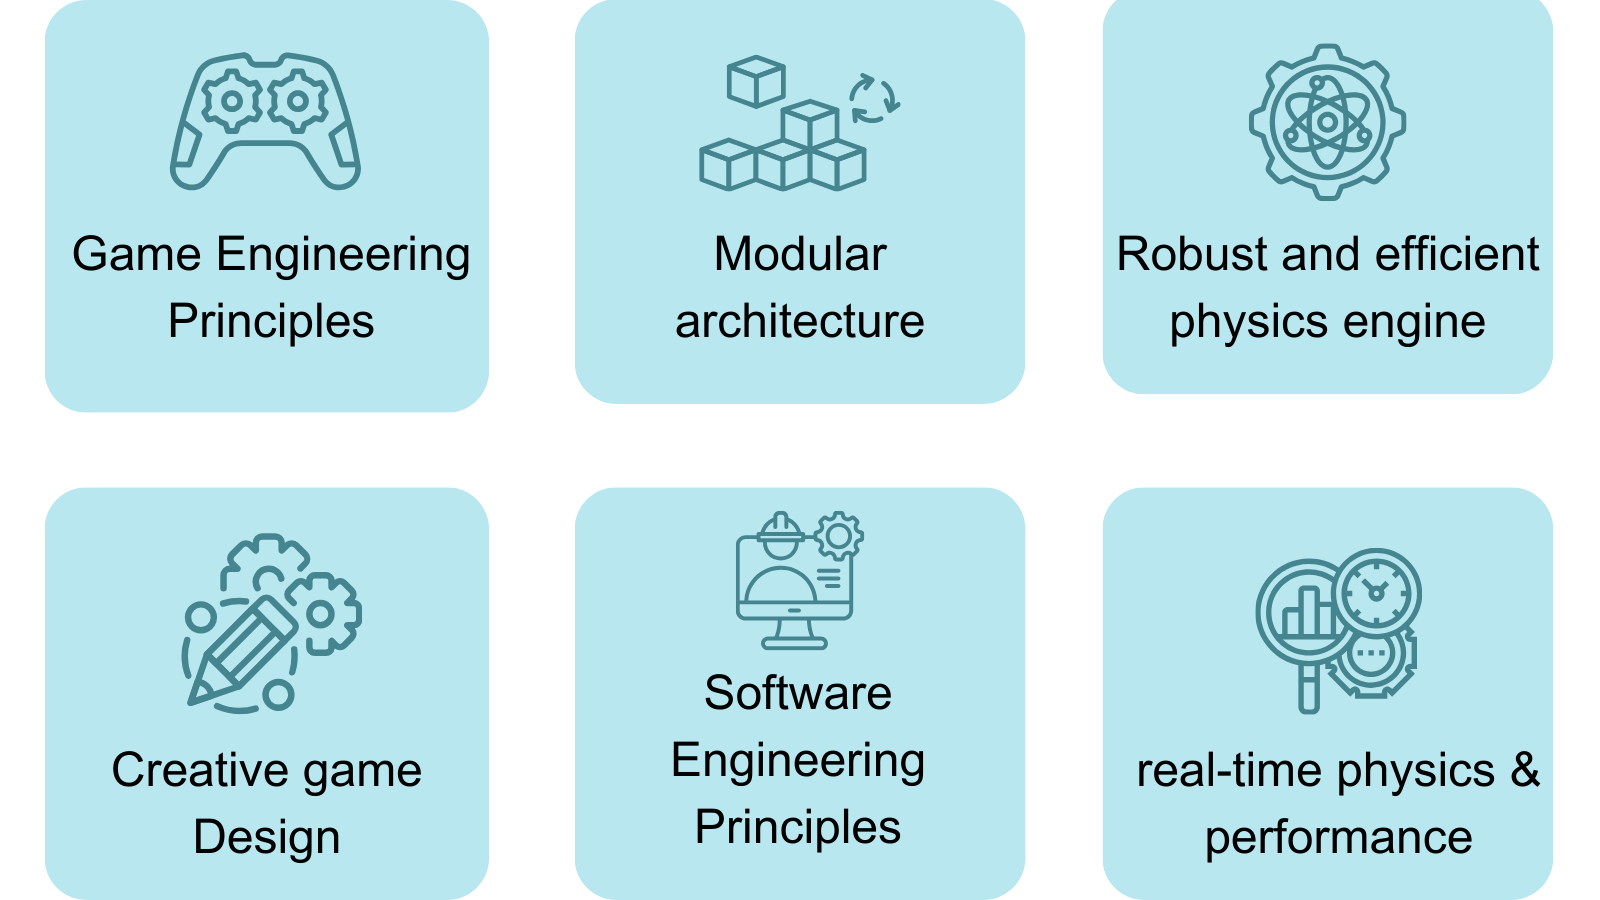
\includegraphics[width=0.65\textwidth]{../figures/focusPoints.png}
    \end{figure}
\end{frame}
% \subsection{Way of working: Scrum and other methodologies}
% Prior to starting the project, we, as a team, devised a project charter that encompasses our vision and mission for the upcoming project.
% Additionally, it includes an analysis of potential challenges and strategies to address them,
% as well as concrete working agreements, including tools to use, style guides and organisational decisions.
% The further development of the game and our collaboration within the team were based on the aforementioned project charter.

% On a weekly basis, a meeting was held with our supervisor.
% During these meetings, the current progress regarding the project timeline, ideas and challenges occurring in development were discussed.
% Furthermore, two time slots were determined each week for a brief discussion of each team member's current work.
% The GitLab \glqq Issues\grqq{} were used to determine feasible work packages, which then could be assigned to one team member.
% Additionally, the Gitlab \glqq Issue Board\grqq{} was used to provide an overview of the progress of each issue.

% Once an issue had been resolved by one team member, a comprehensive review of another team member was required
% before the changes could be incorporated into the mainline.
% This measure was implemented with the objective of guaranteeing code quality and correctness.

% The project's continuous progress was ensured by structuring it in sprints.
% We carried out a total of three sprints, whereby at the beginning of each sprint we defined the objectives at the end of the sprint
% and the issues to be dealt with.

\section{Getting Started}
The project is compatible with Ubuntu 24.04.1 and also supports macOS. 
It includes several bash scripts to simplify installation, running, and testing. 
A platform-agnostic script handles installing dependencies across different operating systems. 
There are separate installation processes for playing the game and for development, with an additional script provided for developers. 
Information on contributing to development can be found in the project documentation \cite{ProjectWiki}.

\subsection{Installing and Running the Game}
To run the game, the script \code{user\_setup.sh} can be used to facilitate the installation of the required packages and dependencies.
In that case, run the following command from the root project directory:

\begin{verbatim}
$ source build-utils/user_setup.sh
\end{verbatim}

%The following packages will be installed based on the operating system:
%\begin{itemize}
%    \item \textbf{Ubuntu:}
%  \code{build-essential cmake xorg-dev libsdl2-dev}
%    \item \textbf{MacOS:}
%  \code{cmake sdl2}.
%\end{itemize}
%The installation of the packages on MacOS requires the use of Homebrew.
%If you do not have it installed you can still run the \code{user\_setup.sh} script, which will install it.

The installation script handles dependencies for both operating systems.
Once all of the dependencies have been installed, the script \code{run.sh} can be executed in order to run the game:
\begin{verbatim}
$ source build-utils/run.sh
\end{verbatim}

\subsection{YAML Configuration}

In this project, a YAML configuration file is used to manage settings and parameters that control various aspects of the game, such as behavior, resources and environmental constants.
The human-readable YAML format allows easy modification of game elements, without the need for recompilation.
This approach enhances development workflow by supporting rapid iterations and testing. The configuration includes:

\begin{itemize}
  \item \textbf{Run Mode and Game Settings:} 
  The configuration begins with a global setting for development mode (\code{run-dev-mode}). 
  When enabled, it provides additional functionality for developers, helping to debug specific components.

  \item \textbf{Assets:} 
  Specifies all audio and visual assets for the game.

  \item \textbf{Items:} 
  Configures game items with their attributes.

  \item \textbf{Landmarks:}
  Defines landmarks, such as the Statue of Liberty or Mount Everest, which act as height references during gameplay.

  \item \textbf{Game Constants:} 
  Includes parameters for in-game mechanics like player movement, health, and environmental interactions. Constants for terrain, item spawning, and physics can be adjusted here, allowing developers to fine-tune gameplay by modifying values such as jump velocity or rock spawn frequency.
\end{itemize}

\subsection{Development Mode}
A dedicated \code{DevMode} is provided, allowing developers to test the game in a controlled environment. This mode bypasses the standard game flow to aid in debugging and fine-tuning specific mechanics.
\pagebreak
\makesection{Game Architecture}

\begin{frame}{Game Architecture}
    \begin{itemize}
        \item Modular design with distinct components for input, physics, rendering, and more.
        \item Game loop structured around core phases:
        \begin{itemize}
            \item Input handling
            \item Physics updates
            \item Rendering updates
        \end{itemize}
    \end{itemize}
    \centering
    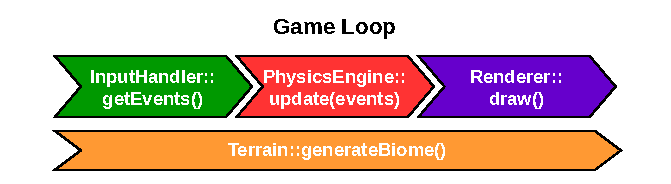
\includegraphics[width=0.6\textwidth]{../figures/physics/gameLoop.pdf} % Insert game loop diagram
\end{frame}
\input{Report-Sections/GameLoop}
\section{The Terrain}
The terrain that the hiker walks on is randomly generated for every game. It is represented by 2D-Splines and is approximated by polylines for collision detection and rendering.

\subsection{Structure}

Internally, the terrain consists of a list of biomes. 
Each biome in turn consists of a list of points $(p_0, p_2, \dots, p_n)$. 
For a reasonably smooth terrain, we decided to use 2D $C^1$-continuous Hermite-Splines to interpolate in between the points. 
Here, every spline interpolates between a start $p_i = (x_i, y_i)^T$ and end point $p_{i+1} = (x_{i+1}, y_{i+1})^T$ given in 2D space. 
To do this, we use separate 1D $C^1$-continuous hermite splines $H_x(t), H_y(t)$ for $x$- and $y$-direction that are both dependent on an artificial third prameter $t$.
This parameter $t$ is roughly equivalent to the distance along the terrain. 
Therefore, it is set to $t_0 = 0$ for the first point and calculated using euclidian distance for every further point.

To get the position of the terrain at a given $t$ we combine the two spline evaluations into a point $(H_x(t), H_y(t))^T$.
We calculate the $C^1$-continuous Hermite-Spline $H_{i,x}(t)$ between a given start and end point $x_{i}, x_{i+1}$ using start and end derivatives $dx_{i}, dx_{i+1}$ and a start value $t_i$ for $t$ as follows. The procedure is analogous for $H_{i,y}(t)$.

% For given start and end points ($(x_s, y_s), (x_e, y_e)$), a given start $t_s$ and given start and end derivatives $(dx_s, dy_s), (dx_e, dy_e)$, we calculate the appropriate splines $H_x(t), H_y(t)$ in the following way:\\
\begin{align}
  t_{i+1} = & t_{i} + \sqrt{(x_{i+1} - x_{i})^2 + (y_{i+1} - y_{i})^2} \\
  H_{i,x}(t) = & (1- 3t^2 + 2t^3)x_{i} + (3t^2 - 2t^3)x_{i+1} \notag\\
  & + (t-2t^2 + t^3)(x_{i+1}-x_{i})dx_{i} \notag\\
  & + (t^3 - t^2)(x_{i+1}-x_{i})dx_{i+1} 
\end{align}

We also experimented with $C^2$-continuous splines. 
In contrast to our method, here the first derivatives at the start and end of a spline are determined by conditions for the second order derivatives and do not need to be provided.
However, these splines typically require us to know all interpolated points at once. 
Consequently, this approach is unsuitable for our generation that is performed in an online manner.
For this reason, we chose to stick with $C^1$-continuous splines and provide the first order derivatives. 

These first order derivatives can be freely chosen but need to match at the borders between splines since the splines are $C^1$-continuous.
Therefore, we provided the start derivative $(dx_0, dy_0)^T = (1, 0)^T$ that corresponds to even terrain. 
From there, we set the derivative of the end of a spline piece to the slope for piecewise linear interpolation:
\begin{align}
  & \forall i\in\{0,1, \dots, n-1\}: \notag\\
  & \quad (dx_{i+1}, dy_{i+1}) = (x_{i+1} - x_i, y_{i+1} - y_i)
\end{align}

The individual spline pieces $H_i(t) = (H_{i, x}(t), H_{i, y}(t))^T$ are then combined into one continuous function $H(t)$, that allows us to interpolate the terrain at any $t$-value between the first and last point.
Using this method, we can generate a spline-based interpolation of the ground points in an online setting which we need for the terrain generation.
%This is particularly useful for the generation of the terrain, where the points are generated iteratively using the existing spline representation.

A good overview over hermite splines is given in \cite{NumerischeGrundlagen2024}.

\subsection{Generation}

At the start of the game, the terrain is generated with one start biome of fixed length. After that, a new biome of the same fixed length is generated whenever the hiker gets close to the right border of the currently generated terrain. 
This is done concurrently to not disturb the playing experience.
Similarly, whenever a biome is no longer visible it is removed from the terrain.

The basepoints used to specify the ground of each biome are generated in an iterative manner.
The overall form of the ground in a biome is specified by the terrain phases $ph_1, ph_2, \dots, ph_n$ of this biome as well as a special starting terrain phase $ph_{s}$ that determines the first few point of the ground.
Here, each terrain phase has the following format: 
\begin{align}
  ph = (\delta v, r, m)
\end{align}
Here, $\delta v \in\R^2$ is the average vector to be added to the last point to generate the next one, $r \in [0,1)$ is the randomness, limiting how much we can rotate the average vector, and $m \in \N$ is the number of points to be generated using this phase before selecting a new phase.

To generate a new point $p_{i+1}$ using the existing terrain up to point $p_i$ and a terrain phase $ph = (\delta v, r, m)$, we first determine the \hyperref[angleRange]{angular range} $[min, max]$ in which generation of a new point is allowed using alg. \ref{alg:maxAngleCalc} for $max$ and its analogon for $min$.
Then, we generate a new point by adding $\delta v$ rotated to a random angle in the range $[min , max]$. 
If the angular range $[min, max]$ is empty, no such point can be generated. 
Therefore, we need to \hyperref[retracing]{retrace} some of the already generated points and try to generate the terrain starting from an earlier point.
%The procedure for generation a new point is described in \hyperref[alg:genNextPoint]{Algorithm \ref{alg:genNextPoint}}.

%{
%
%  \centering
%  \begin{figure}[h]
%  % \begin{minipage}{0.485\textwidth}
%    \vspace{-\abovedisplayskip}
%    \begin{algorithm}[H]
%    \caption{Generating a new point}\label{alg:genNextPoint}
%    \hspace*{\algorithmicindent} \textbf{Input:} $ph = (\delta v, r, m)\in\R^2\times[0,1)\times \N, \, $\\
%    \hspace*{\algorithmicindent} \hphantom{\textbf{Input:}} $p_i\in\R^2, \, terrain\in\left(\R^2\right)^n$\\
%    \hspace*{\algorithmicindent} \textbf{Output:} $p_{i+1}\in \{\bot\}\cup \R^2$
%      \begin{algorithmic}[1]
%      \Procedure{GenerateNextPoint}{$ph, p_i, terrain$}
%      \State $min_a \gets$ \Call{CalculateMinAngle}{$ph, p_i, terrain$}
%      \State $max_a \gets$ \Call{CalculateMaxAngle}{$ph, p_i, terrain$}
%      \If{$min_a = \bot \lor max_a = \bot$}
%        \State \Return $\bot$
%      \EndIf
%      \State $p_{i+1} \gets p_i + $ \Call{RotateRandom}{$\delta v, min_a, max_a$}
%      \State \algorithmiccomment{rotate $\delta v$ by random angle in $[min_a, max_a]$}
%      \State \Return $p_{i+1}$
%      \EndProcedure
%      \end{algorithmic}
%    \end{algorithm}
%  %\end{minipage}
%  \end{figure}
%}
%\vspace{\belowdisplayskip}

{
  \centering
  %\begin{minipage}{0.485\textwidth}
  \begin{figure}[h]
    \vspace{-\abovedisplayskip}
    \begin{algorithm}[H]
    \caption{Calculating the maximum angle}\label{alg:maxAngleCalc}
    \hspace*{\algorithmicindent} \textbf{Input:} $ph = (\delta v, r, m)\in\R^2\times[0,1)\times \N, \, $\\
    \hspace*{\algorithmicindent} \hphantom{\textbf{Input:}} $p_i\in\R^2, \, terrain\in\left(\R^2\right)^n$\\
    \hspace*{\algorithmicindent} \textbf{Output:} $\alpha\in \{\bot\}\cup[-\pi r, \pi r)$
      \begin{algorithmic}[1]
      \Procedure{CalculateMaxAngle}{$ph, p_i, terrain$}
      \State $c_{max} \gets 30; \quad \delta\alpha_{min} \gets 0.01$
      \State $\alpha_{min} \gets -\pi r; \quad \alpha_{max} \gets \pi r$
      \State $\delta\alpha \gets \alpha_{max}; \quad \alpha \gets \alpha_{max}; \quad c \gets 0$
      \While{$(c < c_{max} \land \delta\alpha > \delta\alpha_{min}\land \alpha \leq \alpha_{max})$}
      \State $next\gets p_i + $\Call{Rotate}{$\delta v, \alpha$}
      \If{\Call{FulfillsConstraints}{$p_i, next, terrain$}}
        \State $\delta\alpha \gets \frac{\delta\alpha}{2}$ \algorithmiccomment{lower step size}
        \State $\alpha \gets \alpha + \delta\alpha$
      \Else
        \State $\alpha \gets \alpha - \delta\alpha$ \algorithmiccomment{take back last step}
      \EndIf

      \If{$\alpha \leq \alpha_{min}$} \algorithmiccomment{No $\alpha\in(\alpha_{min}, \alpha_{max}]$ found}
        \State $\alpha \gets \alpha_{max}$
        \State $\delta\alpha \gets \frac{\delta\alpha}{2}$ \algorithmiccomment{Try again with smaller step size}
      \EndIf
      \State $c \gets c + 1$
      \EndWhile

      \State \textbf{if} $c = c_{max}$ \textbf{then} \Return $\bot$ \algorithmiccomment{No viable $\alpha$ found}
      %  \State \Return $\bot$
      %\EndIf

      \State \Return $\alpha - \delta\alpha$ \algorithmiccomment{Restore last viable $\alpha$}
      \EndProcedure
      \end{algorithmic}
    \end{algorithm}
  %\end{minipage}
  \end{figure}
}

\subsubsection{Calculating the angular range}
\label{angleRange}
The angular range in which generation is allowed is defined by a $min$ and $max$ angle which are determined using a bisection method.
% More precisely, we iteratively determine these angles by trying different angles and checking whether the terrain would fulfill the constraints if the new point was generated using the current angle and terrain phase. If so, we can try a larger angle in case of $max$ and a smaller angle in case of $min$.
% The delta angle $\delta_a$ in beween tried angles is halfed for every successful try. If $\delta_a$ gets small enough or we exceed a fixed limit of tries, we return the best previously found angle if one exists or that there is no suitable angle.
This procedure is described in detail for determining $max$ in alg. \ref{alg:maxAngleCalc}.
It is analogous for determining $min$. 
Determining $min$ and $max$ in an example case is illustrated in fig. \ref{pic:calculateAngleRange}.

\imagewithwidth{figures/CalculateAngleRange.pdf}{1.05\columnwidth}{pic:calculateAngleRange}{Calculating the range $[min, max]$ of angles in which the generation of a new point from the last point of the existing terrain and using a given terrain phase $(\delta v, r, m)$ is possible.}{}
\vspace{-\abovedisplayskip}

\subsubsection{Retracing}
\label{retracing}
Although we check all constraints for every generated point, sometimes we cannot generate a new point from the existing terrain. 
Then, we need to retrace parts of the previously generated terrain.
To do so, we remove a fixed number of points from the terrain. 
After that, the generation continues normally. Retracing is illustrated in fig. \ref{pic:retrace}.

\vspace{-\abovedisplayskip}
\imagewithwidth{figures/Retrace.pdf}{\columnwidth}{pic:retrace}{Trying to generate a new point with terrain phase $ph=(\delta v, r, m)$ when the constraints do not allow that. Results in removing of the last few generated points.}{}
\vspace{-\abovedisplayskip}
\newpage
If we cannot regenerate all points that were removed before we retrace again, then we increment how many points need to be removed by a fixed number and retrace again.
We also tried an exponentially increasing retrace count. 
However, that regularly lead to the entire ground being regenerated which took longer overall. Therefore, we decided to use the linearly increasing retrace count.

%\imagewithwidth{figures/Retrace.pdf}{\columnwidth}{pic:retrace}{Trying to generate a new point with the current terrain phase $ph=(\delta v, r, m)$ when the constraints do not allow that. Results in retracing, that is removing of the last few generated points.}{}

%Including the retracing we get the procedure in \hyperref[alg:maxAngleCalc]{Algorithm \ref{alg:genGround}} for generating the ground of a biome of specified length.

%{
%  \centering
%  \begin{figure}[h]
%  %\begin{minipage}{0.485\textwidth}
%    \vspace{-\abovedisplayskip}
%    \begin{algorithm}[H]
%    \caption{Generating the ground of a biome}\label{alg:genGround}
%    \hspace*{\algorithmicindent} \textbf{Input:} $ph_{s} = (\delta v, 0, m) \in\R^2\times\{0\}\times \N, $\\
%    \hspace*{\algorithmicindent} \hphantom{\textbf{Input:}} $phases = \{ph_1, \dots, ph_n | ph_i = $ \\
%    \hspace*{\algorithmicindent} \hphantom{\textbf{Input:}} \hphantom{$phases = \{\}$} $(\delta v_i, r_i, m_i)\in\R^2\times[0,1)\times \N\}$\\
%    %\hspace*{\algorithmicindent} \hphantom{\textbf{Input:}} $phases = \{ph_1, \dots, ph_n | ph_i = (\delta v_i, r_i, m_i)\in\R^2\times[0,1)\times \N\}$\\
%    \hspace*{\algorithmicindent} \hphantom{\textbf{Input:}} $p_0\in \R^2, length \in \R$\\
%    \hspace*{\algorithmicindent} \textbf{Output:} $ground = (p_0, p_1, \dots, p_k) \in (\R^2)^{k+1}$
%      \begin{algorithmic}[1]
%      \Procedure{GenerateGround}{$ph_{s}, phases, p_0, length$}
%      \State $ph \gets ph_{start}, p \gets p_0, t\gets t_0$
%      \State $ground \gets (p_0), phasePointCount \gets 0$
%      \While{$p_x < p_{0,x} + length$}
%        \If{$pointCount = r$} 
%          \State \algorithmiccomment{All points of current phase generated}
%          \State $ph \gets$ \Call{RandomPhase}{$phases$}
%          \State $phasePointCount = 0$
%        \EndIf
%        \State $terrain \gets$ \Call{CalculateTerrain}{$ground$}
%        \State \Comment{\parbox[t]{.8\linewidth}{Terrain within fixed range of last point in $ground$. Needed to check all constraints.}}
%        \vspace{.1cm}
%        \State $p_{new} \gets$ \Call{GenerateNewPoint}{$ph, p, terrain$}
%        \If{$p_{new} = \bot$} \Comment{Can't generate next point}
%          \State \Call{Retrace}{$ground$}
%        \Else
%          \State $ground.add(p_{new})$
%          \State $p \gets p_{new}$
%        \EndIf
%      \EndWhile
%      \State \Return $ground$
%      \EndProcedure
%      \end{algorithmic}
%    \end{algorithm}
%  %\end{minipage}
%\end{figure}
%}

\subsection{Contraints}
\label{constraints}
To determine the angular range for generation and to verify that the newly generated point is appropriate, we formulate several constraints on the terrain.
These constraints ensure that the terrain does not intersect with itself, that there are no too thin parts in the terrain, that it is navigatable by the hiker, and does not generate backwards.
The problems that would arise in the terrain generation should these constraints be violated can be seen in fig. \ref{fig:constraints}.

\begin{figure}[htbp]
  \centering
  \begin{subfigure}{.5\linewidth}
    \centering
    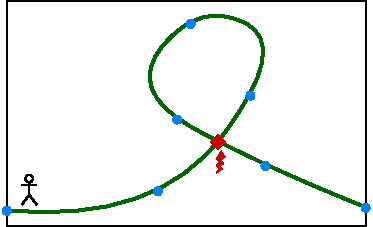
\includegraphics[width=.97\linewidth]{figures/constraints/NoSelfPenetration.pdf}
    \caption{No Selfpenetration}
    \label{pic:noSelfPenetration}
  \end{subfigure}%
  \begin{subfigure}{.5\linewidth}
    \centering
    \includegraphics[width=.97\linewidth]{figures/constraints/minimalBasepointDistance.pdf}
    \caption{Minimal Basepoint Distance}
    \label{pic:minimalBasepointDistance}
  \end{subfigure}

  \vspace{.5cm}
  \begin{subfigure}{.5\linewidth}
    \centering
    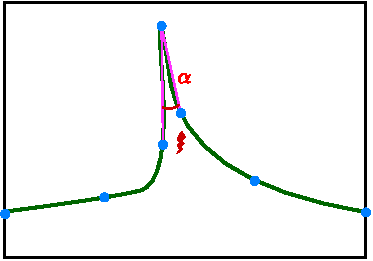
\includegraphics[width=.97\linewidth]{figures/constraints/MinimalBasepointAngle.pdf}
    \caption{Minimal Basepoint Angle}
    \label{pic:minimalBasepointAngle}
  \end{subfigure}%
  \begin{subfigure}{.5\linewidth}
    \centering
    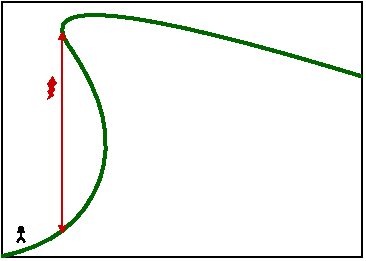
\includegraphics[width=.948\linewidth]{figures/constraints/TerrainJumpeable.pdf}
    \caption{Terrain Jumpable}
    \label{pic:terrainJumpeable}
  \end{subfigure}

  \vspace{.5cm}
  \begin{subfigure}{.5\linewidth}
    \centering
    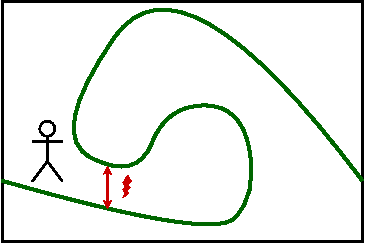
\includegraphics[width=.948\linewidth]{figures/constraints/HikerClearanceHeight.pdf}
    \caption{Hiker Clearance (Height)}
    \label{pic:hikerClearanceHeight}
  \end{subfigure}%
  \begin{subfigure}{.5\linewidth}
    \centering
    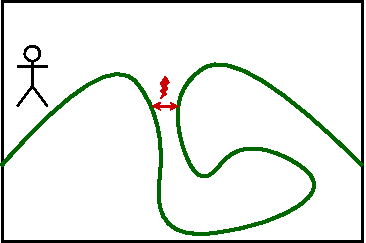
\includegraphics[width=.948\linewidth]{figures/constraints/HikerClearanceWidth.pdf}
    \caption{Hiker Clearance (Width)}
    \label{pic:hikerClearanceWidth}
  \end{subfigure}

  \vspace{.5cm}
  \begin{subfigure}{.5\linewidth}
    \centering
    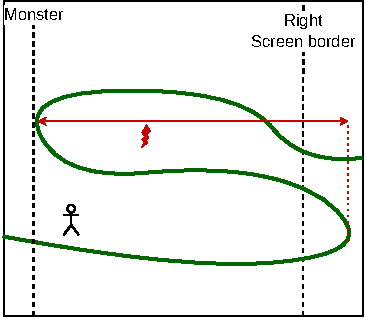
\includegraphics[width=.948\linewidth]{figures/constraints/MaximalOverhangWidth.pdf}
    \caption{Maximal Overhang Width}
    \label{pic:maximalOverhangWidth}
  \end{subfigure}%
  \begin{subfigure}{.5\linewidth}
    \centering
    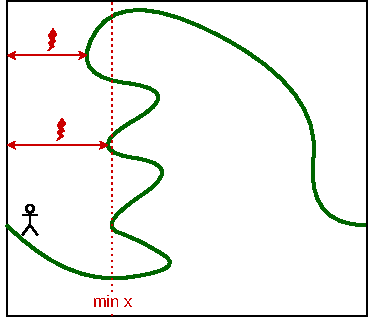
\includegraphics[width=.96\linewidth]{figures/constraints/MinimalXPos.pdf}
    \caption{Minimal x-Pos}
    \label{pic:minimalXPos}
  \end{subfigure}

  \vspace{.3cm}
  \begin{subfigure}{\linewidth}
    \centering
    
\includegraphics[width=\linewidth]{figures/constraints/Legend.pdf}
    %\caption{Legend}
    \label{pic:constraintsLegend}
  \end{subfigure}
  \vspace{-3\abovedisplayskip}
  \caption{Examples of terrains that could be generated if the constraints are ignored.}
  \label{fig:constraints}
  \vspace{-\abovedisplayskip}
\end{figure}
\vspace{-\abovedisplayskip}

%\newpage
\subsection{Representation}

For both rendering and collision detection with rocks and the hiker, the spline-based representation of the terrain is impractical. 
Therefore, the splines are approximated differently for each purpose:

\noindent\textbf{Rendering:}\\
To make the terrain visually appealing, the ground $H(t)$ is approximated by a polyline $T_{rend}$ with a relatively high resolution $res_{rend}$:
\begin{align}
  T_{rend} = & \left(\vphantom{\floor*{\frac{t_n}{res_{rend}} - 1}}H(0), H(res_{rend}), H(2\cdot res_{rend}), \dots, \right. \notag\\
  & \left. H\left(\floor*{\frac{t_n}{res_{rend}} - 1}\cdot res_{rend}\right), H(t_n)\right)
\end{align}

\noindent\textbf{Collision Detection:}\\
To improve performance, the ground is approximated by a polyline $T_{i,cd}$ for each spline-piece $H_i(t)$ using a coarser resolution $res_{cd}$. Combining all of these piecewise approximations into one results in the representation $T_{cd}$ for collision detection:
\begin{align}
  & \forall i\in\{0,1, \dots, n-1\}:\notag\\
  & \quad T_{i, cd} = \left(\vphantom{\floor*{\frac{t_{i+1} - t_i}{res_{cd}} - 1}}\right.H(t_i), H(t_i + res_{cd}), H(t_i + 2\cdot res_{cd}), \dots, \notag\\
  & \quad \hphantom{T_{i, cd} = }\left.H\left(t_i + \floor*{\frac{t_{i+1} - t_i}{res_{cd}} - 1}\cdot res_{cd}\right), H(t_{i+1})\right)
\end{align}
This type of segmented representation is particularly useful for an efficient preselection of relevant terrain sections in the collision detection (see sec. \ref{sec:terrainCD}).
\makesection{Physics}

\begin{frame}{Decoupling Frame Rate and Physics}
    \vspace{-0.25cm}
    \includegraphics<1>[width=\textwidth]{figures/ploop/1.pdf}
    \includegraphics<2>[width=\textwidth]{figures/ploop/2.pdf}
    \includegraphics<3>[width=\textwidth]{figures/ploop/3.pdf}
    \includegraphics<4>[width=\textwidth]{figures/ploop/4.pdf}
    \includegraphics<5>[width=\textwidth]{figures/ploop/5.pdf}
    \includegraphics<6>[width=\textwidth]{figures/ploop/6.pdf}
    \includegraphics<7>[width=\textwidth]{figures/ploop/7.pdf}
    \includegraphics<8>[width=\textwidth]{figures/ploop/8.pdf}
    \includegraphics<9>[width=\textwidth]{figures/ploop/9.pdf}

    \onslide<9>{
        \vspace{-1.1cm}
        \begin{flushright}
            \footnotesize(Fiedler \cite{gafferTimestep})
        \end{flushright}
    }
\end{frame}

\begin{frame}{The Physics Update}
    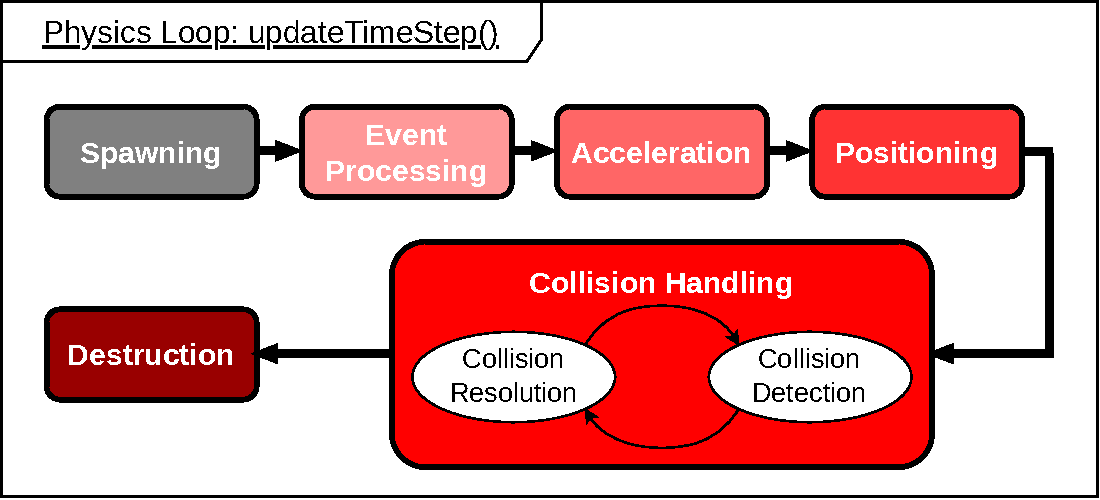
\includegraphics[width=\textwidth]{../figures/physics/updateTimeStep.pdf}
\end{frame}

%\begin{frame}{Colliding Entities}
%    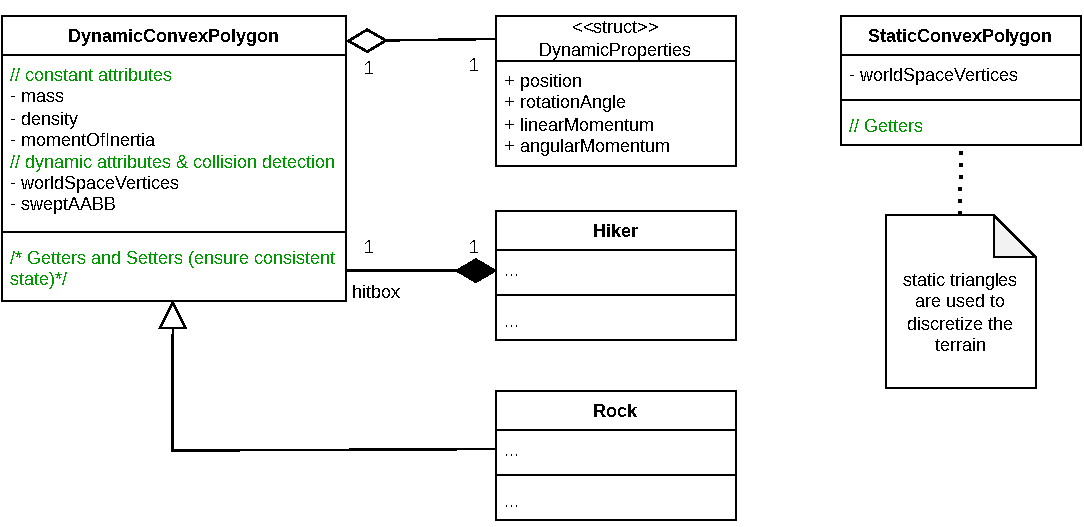
\includegraphics[width=\textwidth]{../figures/physics/rockStateUML3.pdf}
%\end{frame}

\begin{frame}{Movement Equations}
    \begin{itemize}
        \item Based on forces and impulses instead of velocities \cite{baraff}.
        \item Simulated entities have linear and angular momentum.
        \item Movement is governed by:
        \begin{itemize}
            \item Gravitational force (body force)
            \item Collision impulses (surface impulses)
        \end{itemize}
        \item System of continuous ODEs is discretized with the symplectic euler method.
    \end{itemize}
    \begin{minipage}{\textwidth}
        \centering
        \begin{minipage}{.495\textwidth}
            \begin{align*}
                \frac{\textbf{d}}{\textbf{d}{t}} 
                \left(
                  \begin{array}{c}
                    \overrightarrow{x}(t)\\
                    \overrightarrow{P}(t)\\
                    \theta(t)\\
                    L(t)
                  \end{array}
                \right)
                =
                \left(
                  \begin{array}{c}
                    {\overrightarrow{P}(t)}/{m}\\
                    \overrightarrow{F}(t)\\
                    L(t)/I\\
                    \tau(t)
                  \end{array}
                \right)
            \end{align*}
        \end{minipage}
        \begin{minipage}{.495\textwidth}
            \begin{align*}
                \overrightarrow{P}^{t+1} &= \overrightarrow{P}^{t} + \delta t \cdot \overrightarrow{F}^{t}\\
                \overrightarrow{x}^{t+1} &= \overrightarrow{x}^{t} + \delta t \cdot \frac{\overrightarrow{P}^{t+1}}{m}\\
                L^{t+1} &= L^{t} + \delta t \cdot \tau^{t}\\
                \theta^{t+1} &= \theta^{t} + \delta t \cdot \frac{L^{t+1}}{I}
              \end{align*}
        \end{minipage}
    \end{minipage}
\end{frame}

\begin{frame}{Collision Detection: Broadphase (swept AABBs \cite{sweptAABB})}
  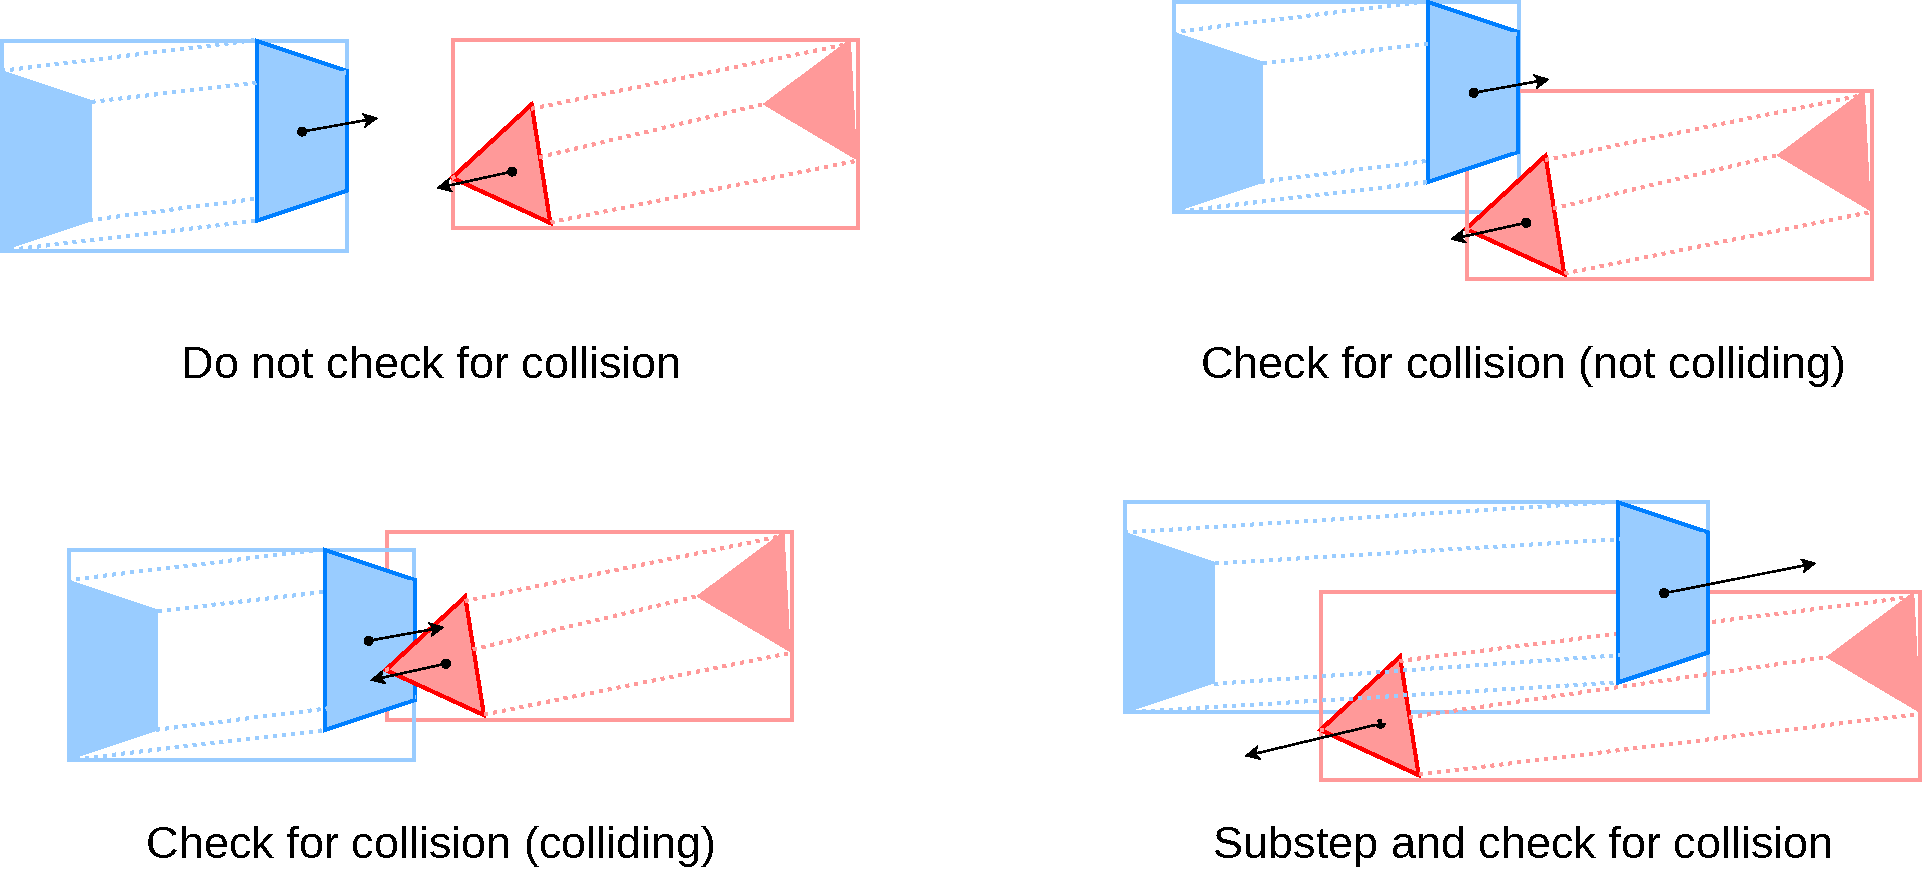
\includegraphics[width = \textwidth]{../figures/physics/aabb_extended.pdf}
\end{frame}

\begin{frame}{Collision Detection: Narrowphase (SAT \cite{geometrySAT})}
    \centering
    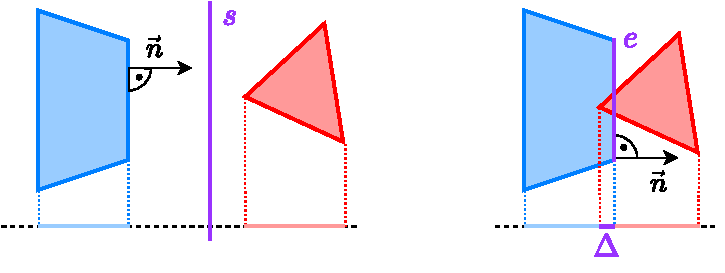
\includegraphics[width = \textwidth]{../figures/physics/sat2.pdf}
\end{frame}

\begin{frame}{Collision Resolution}
    \begin{figure}
        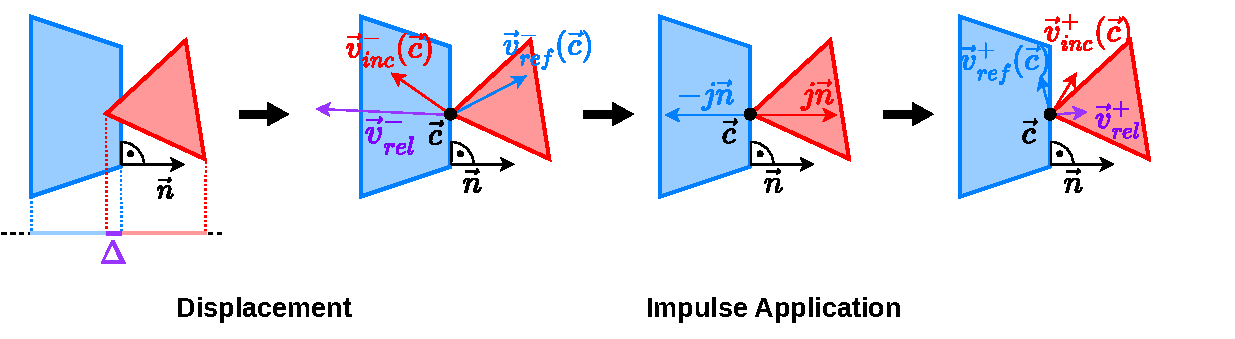
\includegraphics[width = \textwidth]{../figures/physics/resolution2.pdf}
    \end{figure}
    \begin{itemize}
        \item Empirical Law for Frictionless Collisions \cite{baraff}: $\left<\overrightarrow{v}_{rel}^{\,+}, \overrightarrow{n}\right> = -\epsilon\left<\overrightarrow{v}_{rel}^{\,-}, \overrightarrow{n}\right>$
        \item $\epsilon$ is the coefficient of restitution (``bounciness factor'')
    \end{itemize}
\end{frame}

\begin{frame}{Types of Collisions}
    \begin{minipage}{\textwidth}
        \centering
        \begin{minipage}{0.24\textwidth}
            \centering
            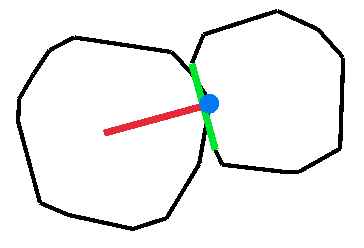
\includegraphics[width=\textwidth]{figures/colls/rrw.png}
        \end{minipage}
        \begin{minipage}{0.24\textwidth}
            \centering
            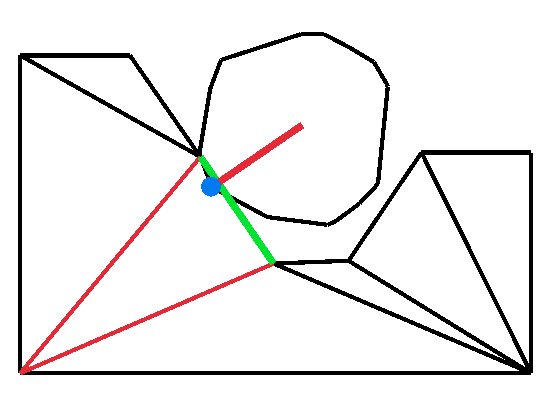
\includegraphics[width=\textwidth]{figures/colls/rtw.png}
        \end{minipage}
        \begin{minipage}{0.24\textwidth}
            \centering
            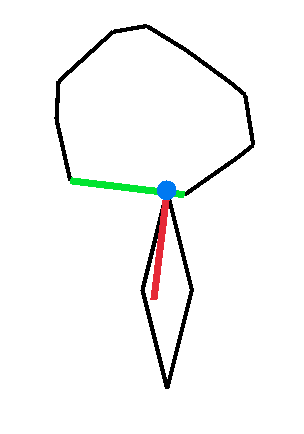
\includegraphics[width=.8\textwidth]{figures/colls/rhw.png}
        \end{minipage}
        \begin{minipage}{0.24\textwidth}
            \centering
            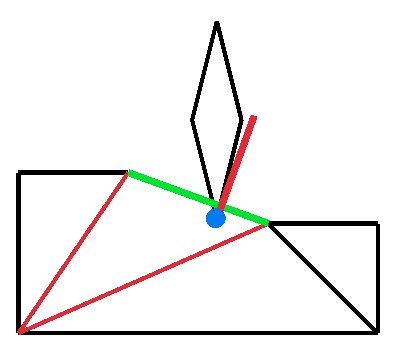
\includegraphics[width=\textwidth]{figures/colls/htw.png}
        \end{minipage}
    \end{minipage}
    \begin{minipage}{\textwidth}
        \centering
        \begin{minipage}{0.24\textwidth}
            \centering
            Rock-Rock
        \end{minipage}
        \begin{minipage}{0.24\textwidth}
            \centering
            Rock-Terrain
        \end{minipage}
        \begin{minipage}{0.24\textwidth}
            \centering
            Rock-Hiker
        \end{minipage}
        \begin{minipage}{0.24\textwidth}
            \centering
            Hiker-Terrain
        \end{minipage}
    \end{minipage}
\end{frame}

\begin{frame}{Performance Considerations}
    \begin{itemize}
        \item Performance optimizations for handling large numbers of entities.
        \item Usage of swept AABBs prunes collision checks with SAT.
        \item Warm starting to further reduce cost of the SAT algorithm.
        \item Pre-computation of world-space coordinates and AABBs upon moving an entity instead of during every collision check.
        \item Effective garbage collection for entities and terrain that leave the scope of the game.
    \end{itemize}
    \centering
    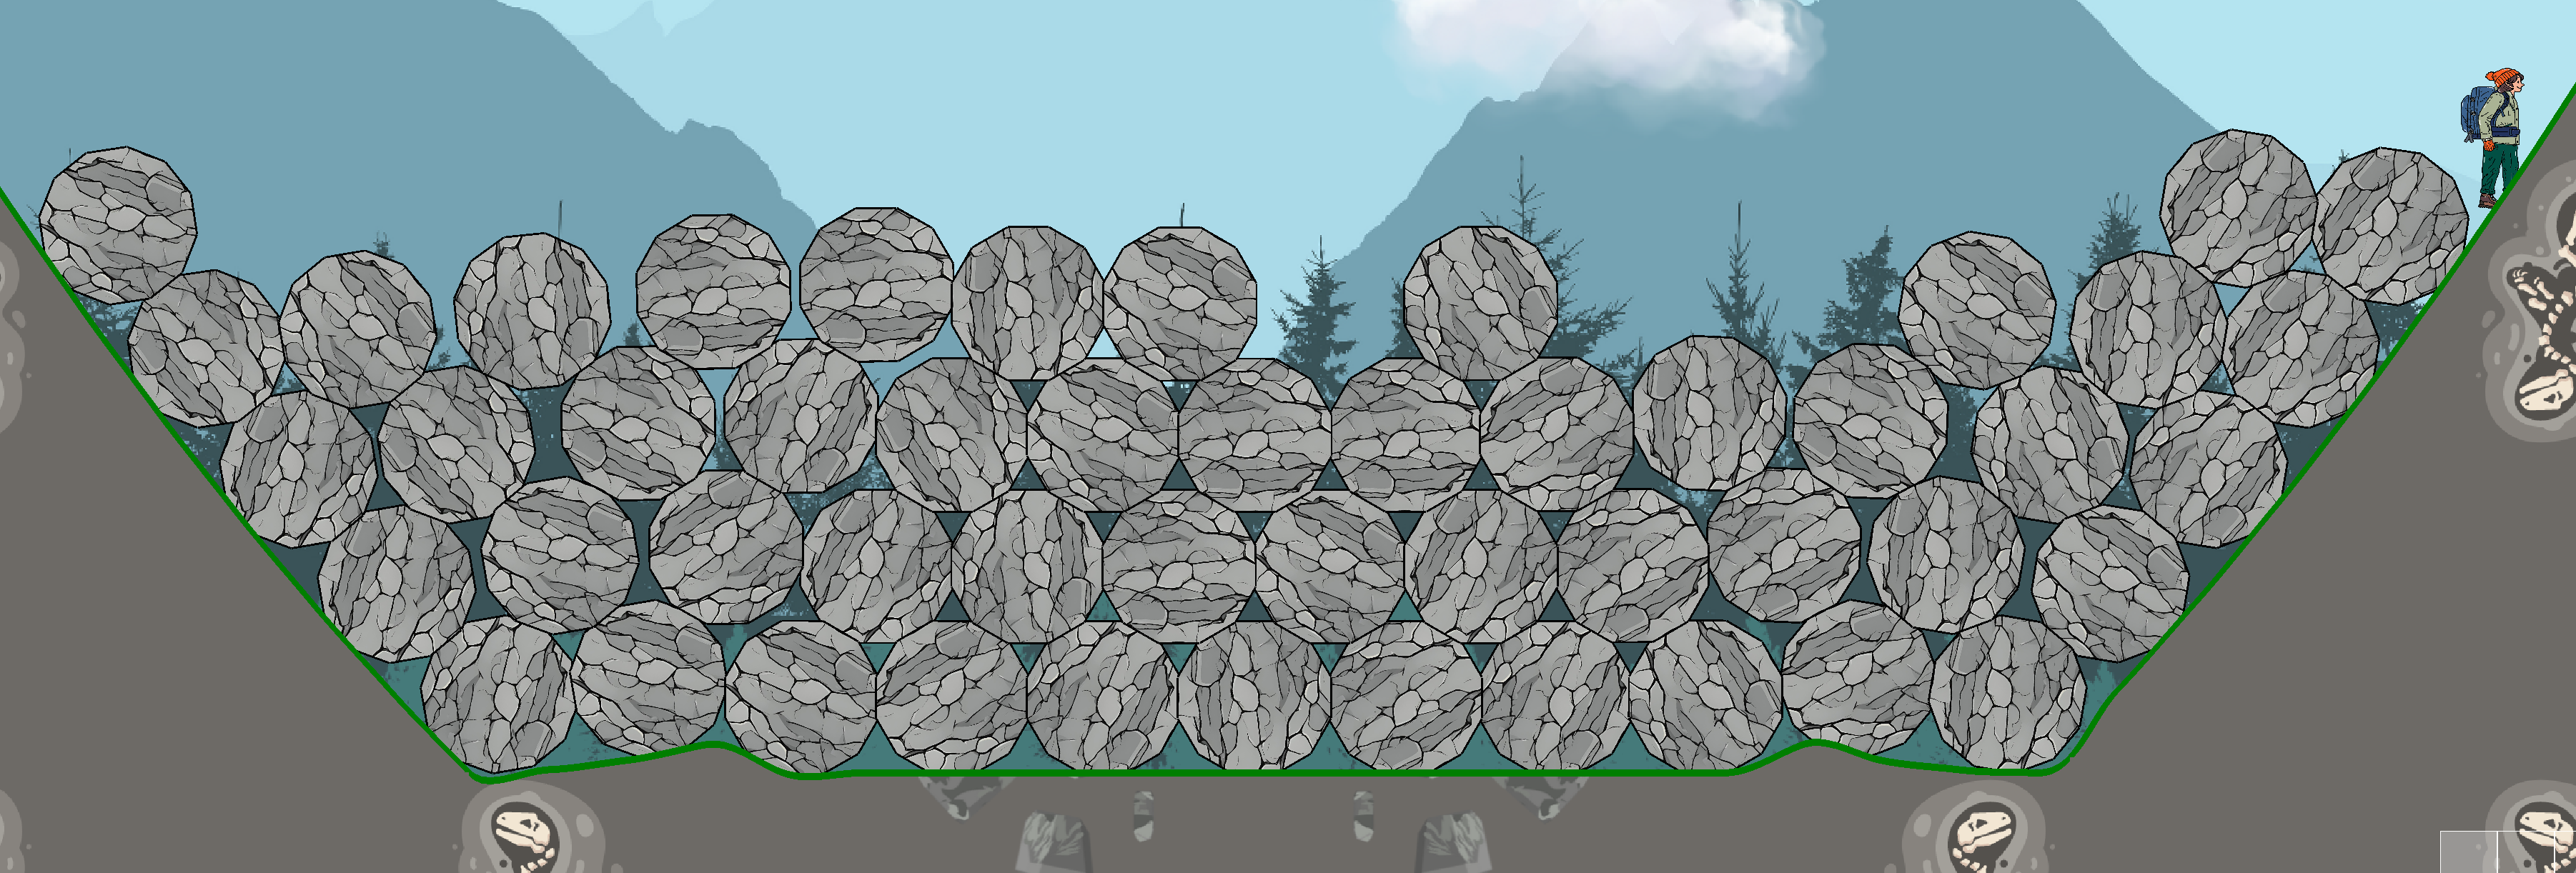
\includegraphics[width=.6\textwidth]{figures/sim.png}
\end{frame}
\makesection{Rendering}

\begin{frame}{Rendering Architecture}
    \centering
    % Define the style for the boxes
    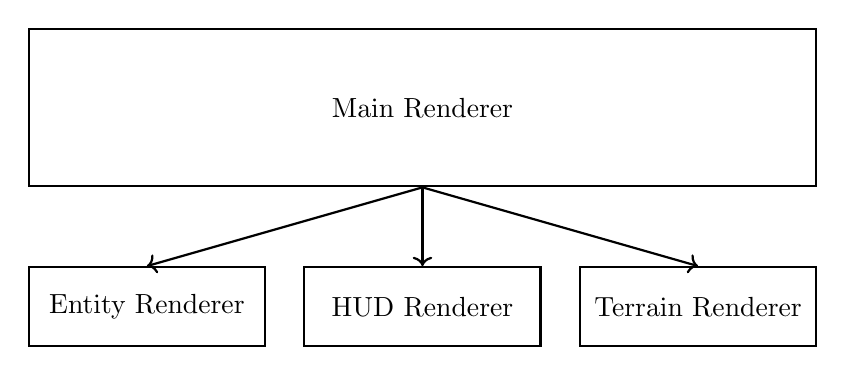
\begin{tikzpicture}
        % Main Renderer
        \node[draw, thick, minimum width=10cm, minimum height=2cm] (main) {Main Renderer};

        % Subrenderers: TerrainRenderer, HUDRenderer, EntityRenderer
        \node[draw, thick, minimum width=3cm, minimum height=1cm, below=1cm of main, xshift=-3.5cm] (entity) {Entity Renderer};
        \node[draw, thick, minimum width=3cm, minimum height=1cm, below=1cm of main] (hud) {HUD Renderer};
        \node[draw, thick, minimum width=3cm, minimum height=1cm, below=1cm of main, xshift=3.5cm] (terrain) {Terrain Renderer};

        % Arrows from main renderer to subrenderers
        \draw[->, thick] (main.south) -- (entity.north);
        \draw[->, thick] (main.south) -- (terrain.north);
        \draw[->, thick] (main.south) -- (hud.north);
    \end{tikzpicture}
\end{frame}

\begin{frame}{Rendering Architecture - Normal Mode}
    \centering
    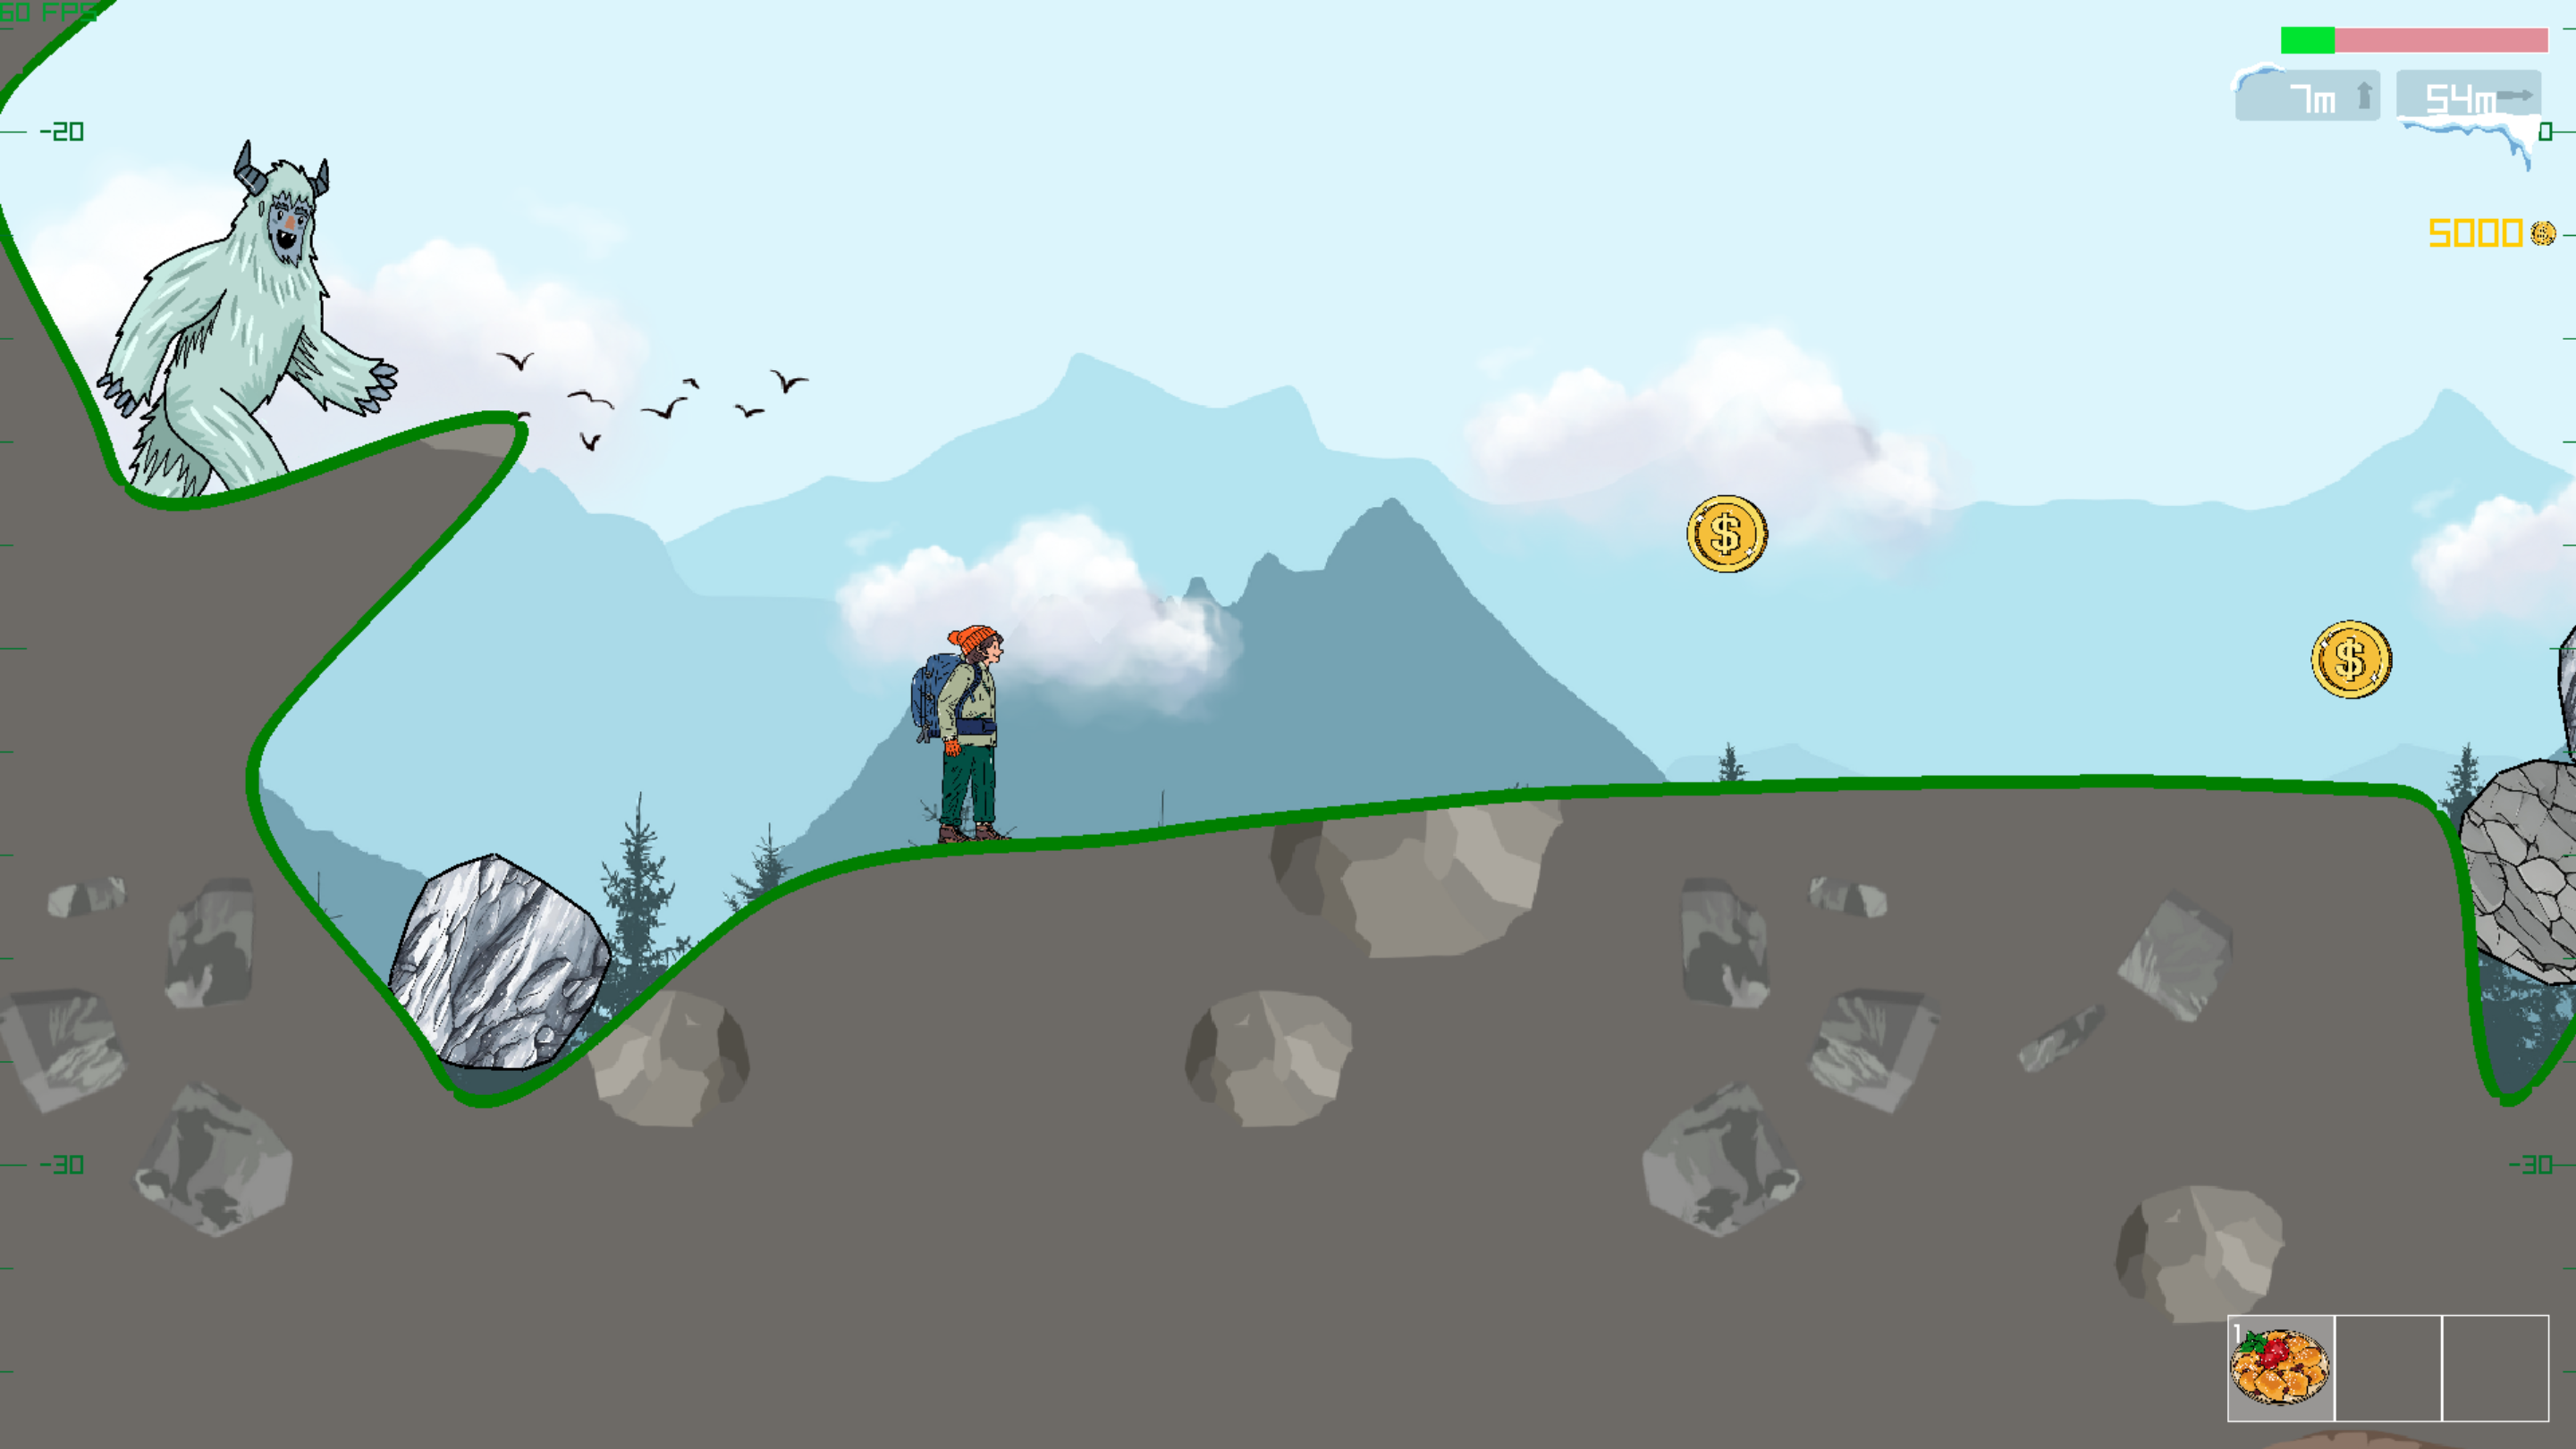
\includegraphics[width=0.85\textwidth]{../figures/Ingame-Picture.png}
\end{frame}

\begin{frame}{Rendering Architecture}
    \begin{tabular}{ccc}

        \parbox{0.3\textwidth}{
            \centering \textbf{Entity Renderer}
            \vspace{0.2cm}
            \begin{itemize}
                \item Entities are rendered with their respective textures
                \item Handles animations of the entities, e.g. walking
            \end{itemize}
            \vspace{0.5cm}
            \centering
            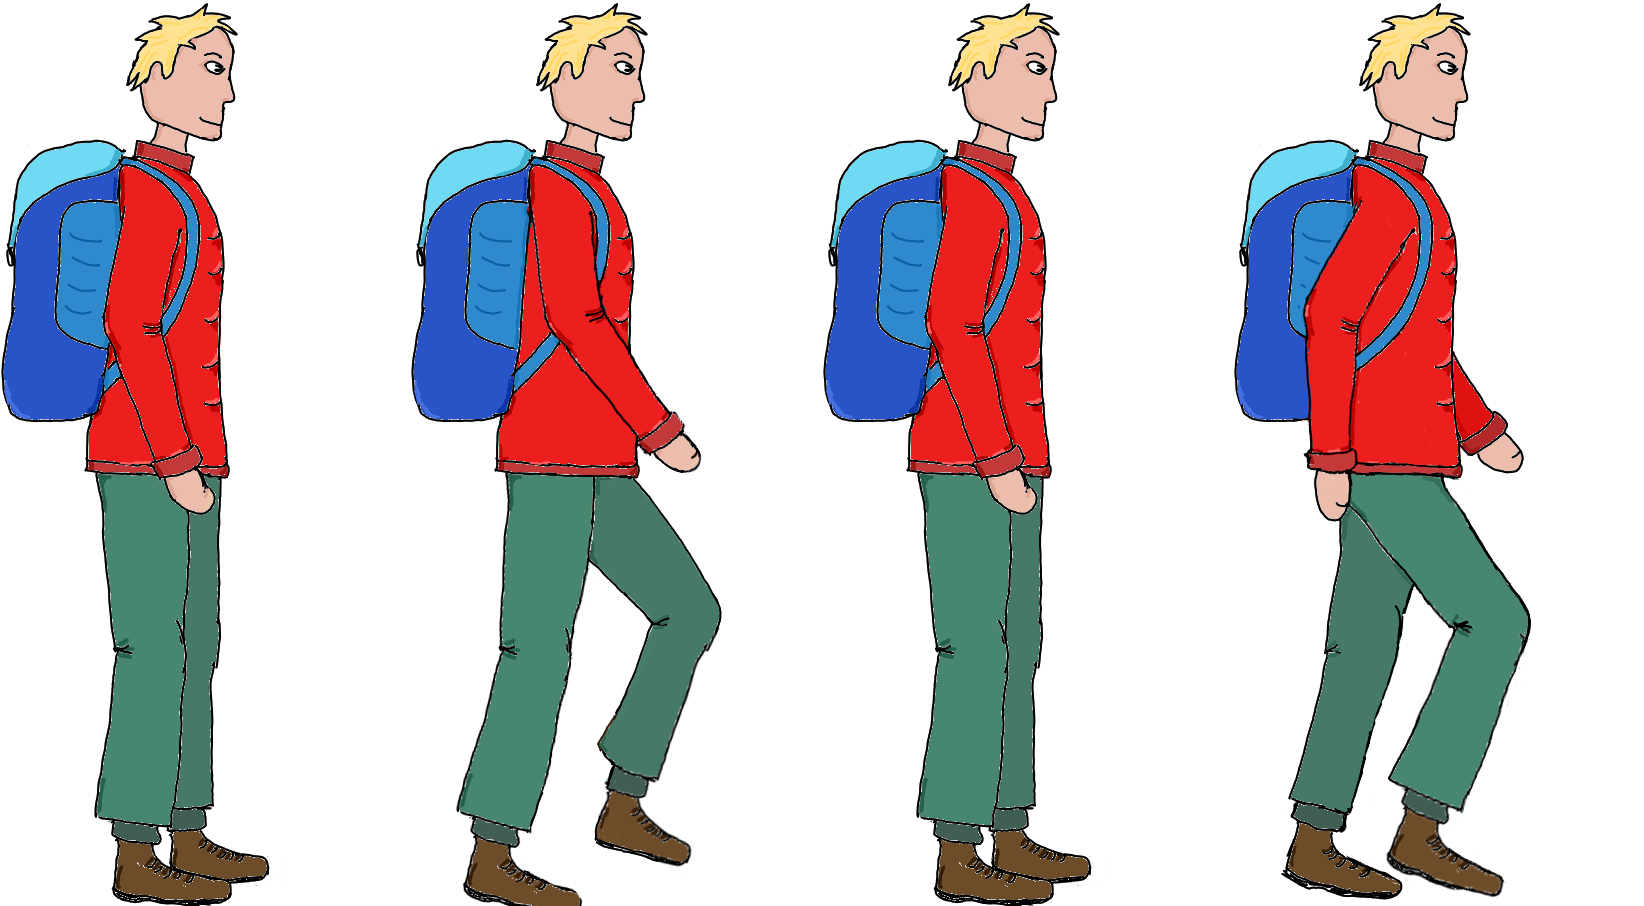
\includegraphics[width=0.25\textwidth]{../../assets/texture/player_walk.png}
        } &

        \pause
        
        \parbox{0.3\textwidth}{
            \centering \textbf{Terrain Renderer}
            \vspace{0.2cm}
            \begin{itemize}
                \item Terrain is continuously rendered with a texture
            \end{itemize}
            \vspace{0.5cm}
            \centering
            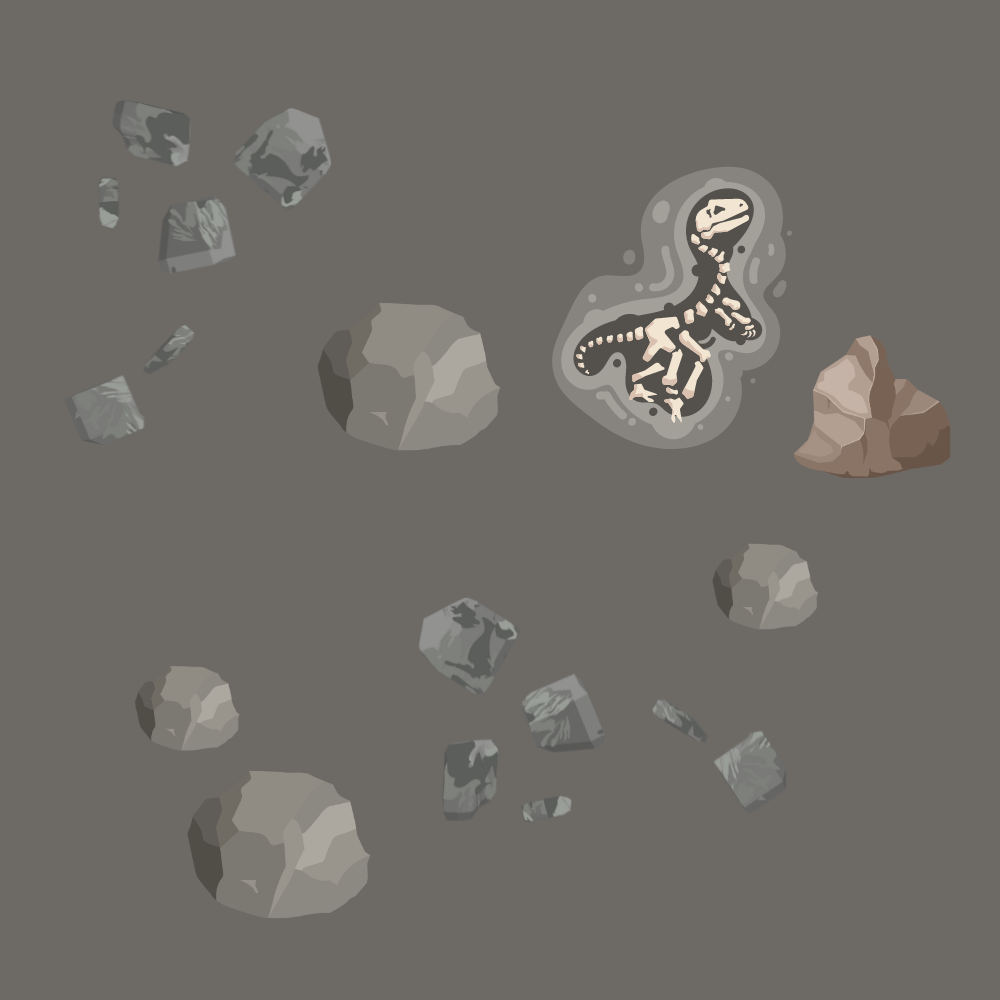
\includegraphics[width=0.2\textwidth]{../../assets/layers/mountain3.png}
        } &

        \pause
        
        \parbox{0.3\textwidth}{
            \centering \textbf{HUD Renderer}
            \vspace{0.2cm}
            \begin{itemize}
                \item Heads-Up-Display (HUD) is rendered on top of the game
                \item Displays the player's health, score, inventory, etc.
            \end{itemize}
            \vspace{0.5cm}
            \centering
            \begin{tabular}{ccc}
                
\includegraphics[width=0.07\textwidth]{../../assets/texture/coin.png} &
                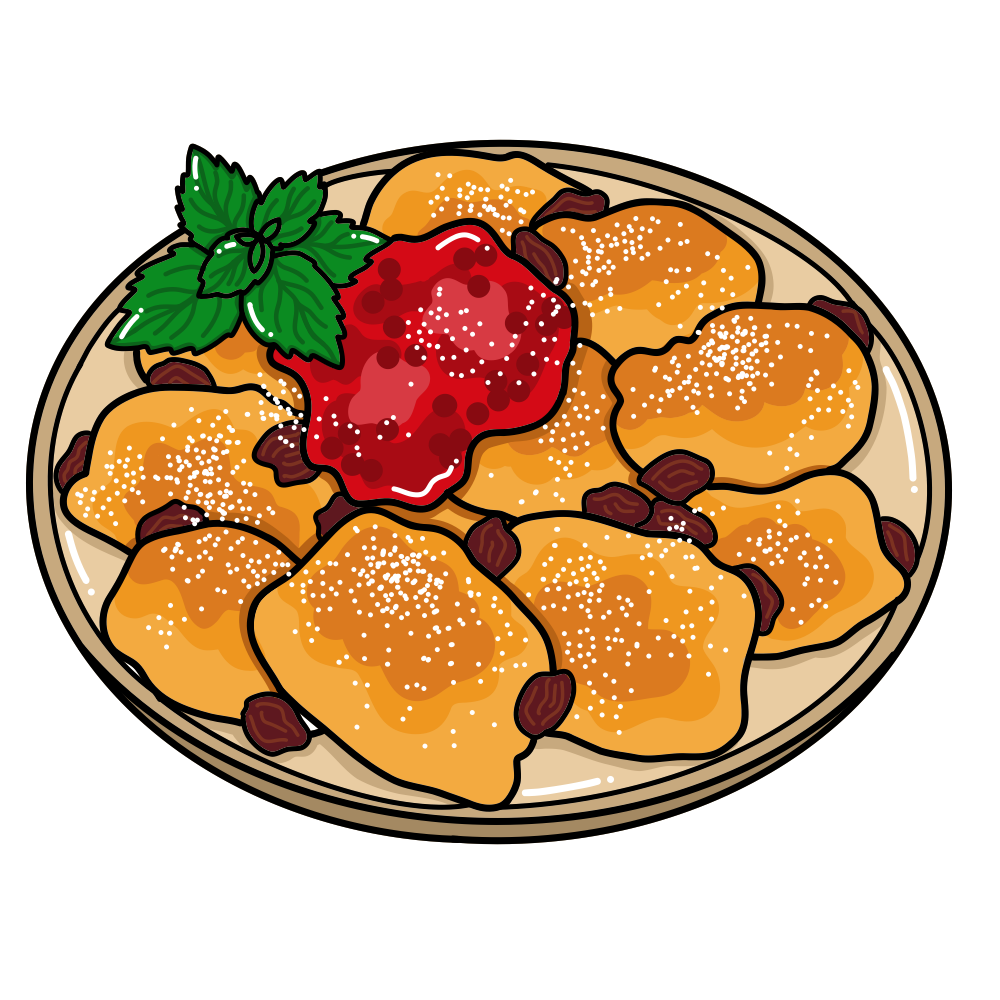
\includegraphics[width=0.07\textwidth]{../../assets/texture/kaiserschmarrn.png} &
                
\includegraphics[width=0.07\textwidth]{../../assets/texture/duck.png}
            \end{tabular}
        }
    \end{tabular}
\end{frame}




\begin{frame}{Rendering Architecture - Debug Mode}
    \centering
    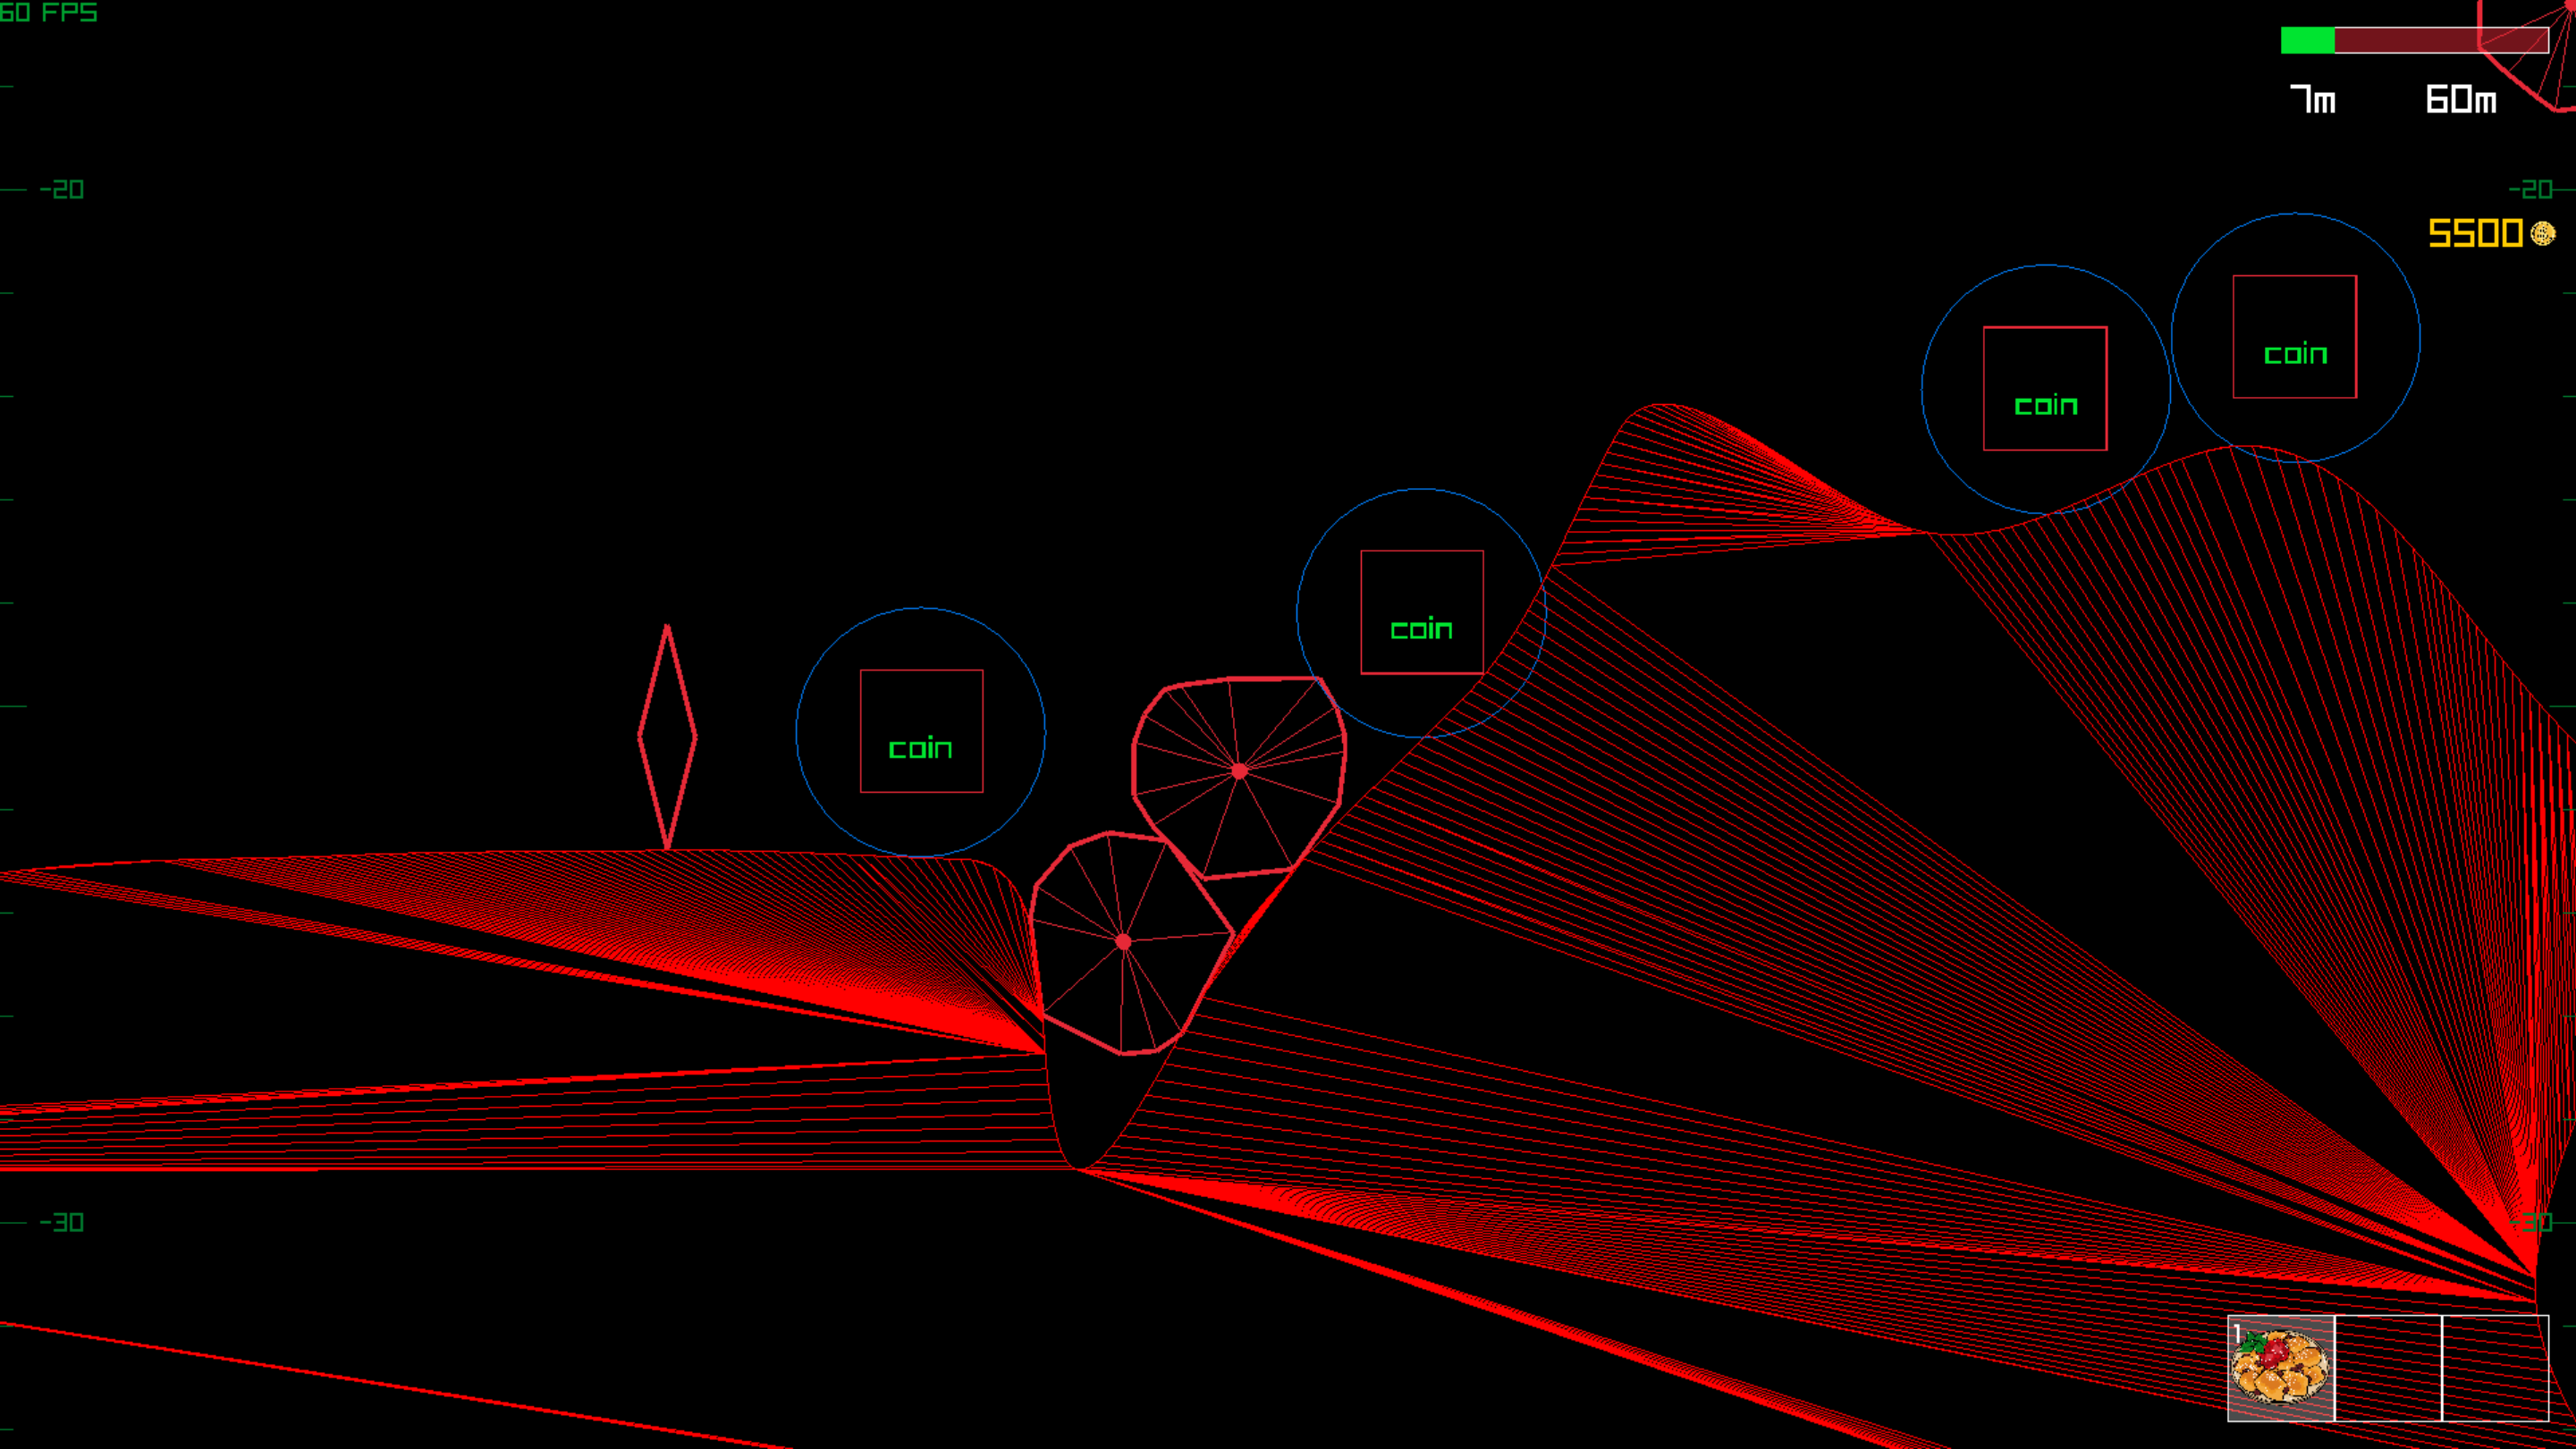
\includegraphics[width=0.85\textwidth]{../figures/Debug-Mode.png}
\end{frame}
\makesection{Conclusion}

\begin{frame}{Conclusion and Future Work}
    \begin{itemize}
        \item Achievements:
        \begin{itemize}
            \item Modular architecture and optimized codebase
            \item Enhanced user experience with new features
        \end{itemize}
        \item Proposed future expansions:
        \begin{itemize}
            \item Multiplayer modes and leaderboard integration
            \item New game items and biomes
            \item Enhanced physics with friction, air resistance, and more
        \end{itemize}
    \end{itemize}
\end{frame}
\section{Future Work}

While our implementation represents a significant step forward, the project offers ample opportunity for future expansion. %, including optimization of the physics engine, exploration of new biomes, items and game modes, and introduction of multiplayer capabilities. 
%Although our implementation could have been more performant had we used flecs, we opted for a design that allows continuous forwards-facing evolution of the game and is easy to work with for us and possibly other developers.
%
Therefore, we want to mention some concrete examples and ideas that can be used as starting point for the further development.
New items can be added such as a pickaxe or a gun that can shatter rocks.
Competitiveness between players could be introduced with a leaderboard.
Different biomes with different visuals and terrain generation can be implemented.  
Another option is to offer difficulty settings to the user and implementing a coin shop for buying upgrades.
Moreover, we propose a multiplayer mode where there are two hikers competing for who gets furthest and interacting with each other.
Alternatively, one player could play as the monster and throw snowballs at the hiker.
%The implementation of this mode requires the consideration of how players interact and how to resolve several aspects, e.g. the potential for player interaction and the resolution of scenarios such as the death of one player.

Our physics engine also offers various extension points.
One known issue with the way our physics are currently implemented is that we assume there are only vertex-face collisions as shown in fig. \ref{fig:SAT}.
However, edge-edge collisions can occur resulting in a jittering effect when rocks are stationary on the ground (see fig. \ref{fig:jitter}) due to falsely introduced torque.
Although this does not constitute a problem for our bouncy physics right now, we are aware that this will need to be solved if the game is to be extended with less bouncy entities.
Catto \cite{cattoManifolds} and Wheeler \cite{wheelerCD} show how to handle this effect using \emph{collision manifolds}.
The idea is to consider up to two colliding points between polygons and applying a combined impulse at an average contact point of the two colliding points weighed by their collision depth.

Another way of extending the physics engine would be to add friction or air resistance.
Friction can be modelled as two constants for static and dynamic friction.
A friction impulse is then applied during collisions in reverse tangential direction to $\vec{v}_{rel}$.
For the magnitude, simply replace the normal $\vec{n}$ with the tangent $\vec{t}$ in equation \ref{eq:scary}.
We implemented friction but decided against using it as it would currently negatively impact gameplay, which requires bouncy rocks.

Lastly, there are opportunities to further enhance the performance of the physics engine, e.g. by implementing parallel batch processing and spatial data structures.

% \subsection{Future Work}

% The physics engine we developed is suitable for our purpose and can be easily extended.



% To summarize, our physics engine provides a modular and highly extensible framework that can be built upon in many ways.
% It is suitable for small games and can be easily adapted to any small game that needs to simulate rigid convex polygons.

\begin{figure}[h!]
  \centering
  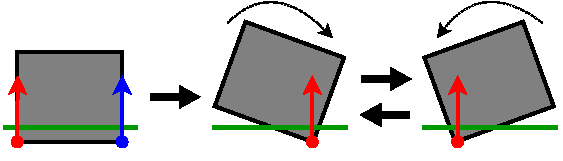
\includegraphics[width = .7\linewidth]{figures/physics/jitter.pdf}
  \caption{An edge-edge collision should consider more than one contact point in order to accurately resolve the collision. Here, the blue collision point is ignored and jitter is introduced.}
  \label{fig:jitter}
\end{figure}

% if have a single appendix:
%\appendix[Proof of the Zonklar Equations]
% or
%\appendix  % for no appendix heading
% do not use \section anymore after \appendix, only \section*
% is possibly needed

% use appendices with more than one appendix
% then use \section to start each appendix
% you must declare a \section before using any
% \subsection or using \label (\appendices by itself
% starts a section numbered zero.)
%


%\appendices
%\section{Proof of the First Zonklar Equation}
%Appendix one text goes here.

% you can choose not to have a title for an appendix
% if you want by leaving the argument blank
%\section{}
%Appendix two text goes here.


% use section* for acknowledgment
%\ifCLASSOPTIONcompsoc
  % The Computer Society usually uses the plural form
%  \section*{Acknowledgments}
%\else
  % regular IEEE prefers the singular form
%  \section*{Acknowledgment}
%\fi


%The authors would like to thank...


% Can use something like this to put references on a page
% by themselves when using endfloat and the captionsoff option.
\ifCLASSOPTIONcaptionsoff
  \newpage
\fi



% trigger a \newpage just before the given reference
% number - used to balance the columns on the last page
% adjust value as needed - may need to be readjusted if
% the document is modified later
%\IEEEtriggeratref{8}
% The "triggered" command can be changed if desired:
%\IEEEtriggercmd{\enlargethispage{-5in}}

% references section

% can use a bibliography generated by BibTeX as a .bbl file
% BibTeX documentation can be easily obtained at:
% http://mirror.ctan.org/biblio/bibtex/contrib/doc/
% The IEEEtran BibTeX style support page is at:
% http://www.michaelshell.org/tex/ieeetran/bibtex/
\bibliographystyle{IEEEtran}
% argument is your BibTeX string definitions and bibliography database(s)
\bibliography{bib/literatur.bib}{}
%
% <OR> manually copy in the resultant .bbl file
% set second argument of \begin to the number of references
% (used to reserve space for the reference number labels box)
% \begin{thebibliography}{1}
% \end{thebibliography}

% biography section
% 
% If you have an EPS/PDF photo (graphicx package needed) extra braces are
% needed around the contents of the optional argument to biography to prevent
% the LaTeX parser from getting confused when it sees the complicated
% \includegraphics command within an optional argument. (You could create
% your own custom macro containing the \includegraphics command to make things
% simpler here.)
%\begin{IEEEbiography}[{\includegraphics[width=1in,height=1.25in,clip,keepaspectratio]{mshell}}]{Michael Shell}
% or if you just want to reserve a space for a photo:

%\begin{IEEEbiography}{Michael Shell}
%Biography text here.
%\end{IEEEbiography}

% if you will not have a photo at all:
%\begin{IEEEbiographynophoto}{John Doe}
%Biography text here.
%\end{IEEEbiographynophoto}

% insert where needed to balance the two columns on the last page with
% biographies
%\newpage

%\begin{IEEEbiographynophoto}{Jane Doe}
%Biography text here.
%\end{IEEEbiographynophoto}

% You can push biographies down or up by placing
% a \vfill before or after them. The appropriate
% use of \vfill depends on what kind of text is
% on the last page and whether or not the columns
% are being equalized.

%\vfill

% Can be used to pull up biographies so that the bottom of the last one
% is flush with the other column.
%\enlargethispage{-5in}



% that's all folks
% \end{document}

\end{document}